\documentclass[11pt]{article}

% Encoding and font setup
\usepackage[T1]{fontenc}
\usepackage[utf8]{inputenc}
\usepackage{lmodern}

% Page layout and micro-typography
\usepackage[margin=1in]{geometry}
\usepackage{microtype}
\usepackage{csquotes}
\usepackage{float} % for [H] exact placement of figures
\usepackage[section]{placeins} % prevent floats from crossing section boundaries
\usepackage[skip=0pt]{caption} % control caption spacing

% Math and figures
\usepackage{amsmath, amssymb}
\usepackage{graphicx}
\graphicspath{{../images/}} % look for images in the images/ folder one level up

% Remove vertical whitespace around figures
\setlength{\intextsep}{0pt}
\setlength{\textfloatsep}{0pt}
\setlength{\floatsep}{0pt}
\setlength{\dbltextfloatsep}{0pt}
\setlength{\dblfloatsep}{0pt}
\setlength{\abovecaptionskip}{0pt}
\setlength{\belowcaptionskip}{0pt}
\captionsetup[figure]{aboveskip=0pt, belowskip=0pt}

% Links
\usepackage{hyperref}
\hypersetup{colorlinks=true, linkcolor=blue, urlcolor=blue, citecolor=blue}

% Title information
\title{Project Type Synthesis Homework}
\author{Peyton Lettau, Sebastian Hondl, John Robinson, Will McConnell}
\date{\today}

\begin{document}

\maketitle

\tableofcontents
\newpage

\section{US4509509A: Apparatus for Treating the Joints of the Human Body}
\subsection{Description}
CPM apparatus that reciprocates a joint while coordinating electrical muscle stimulation; travel-path switches energize a stimulator during selected phases and directions of motion to contract target muscles in sync with flexion/extension.
\subsection{Images}
\begin{figure}[H]
  \centering
  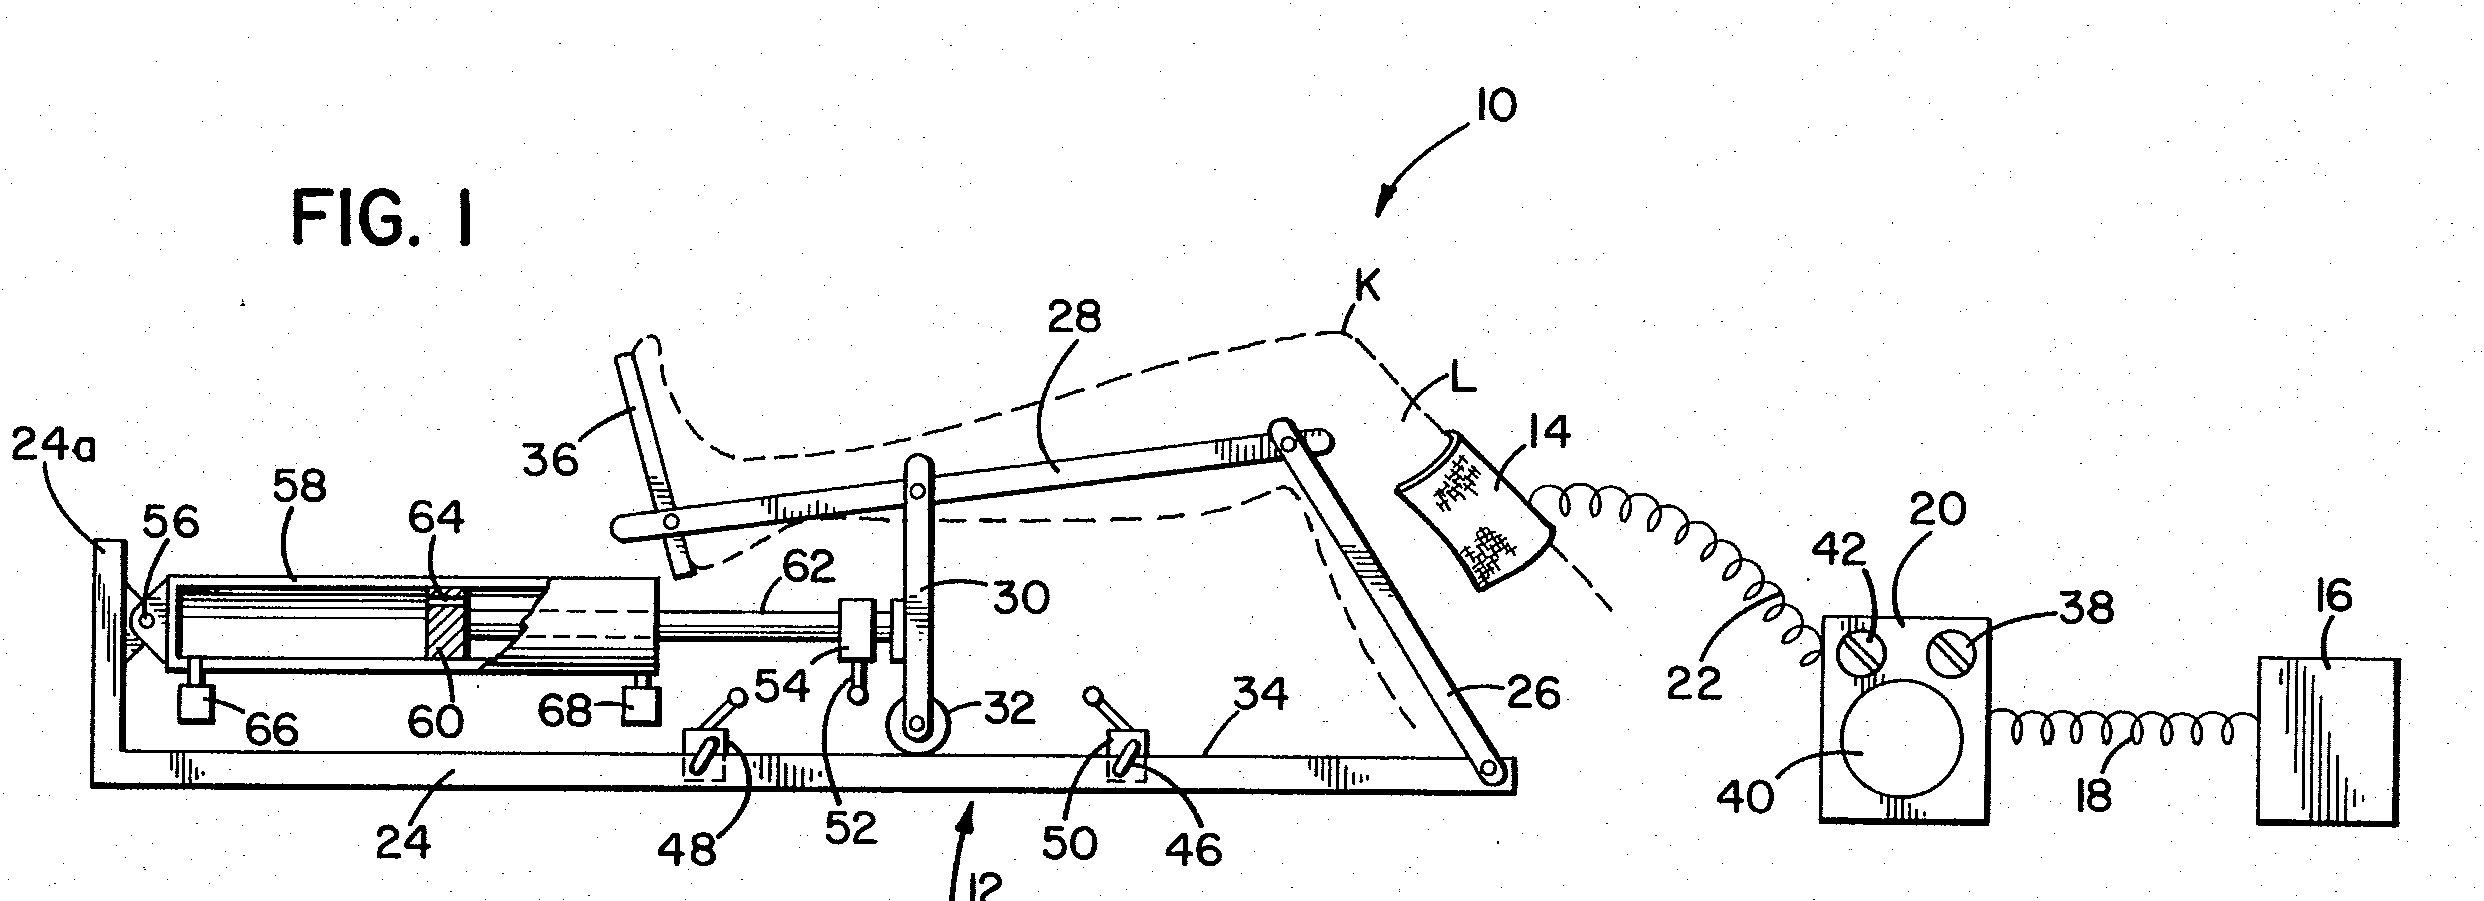
\includegraphics[width=0.54\linewidth]{US4509509.png}
  \caption{US4509509A apparatus illustrating adjustable thigh/calf supports and drive linkage.}
  \label{fig:US4509509A}
\end{figure}

\subsection{Mechanism kinematics}
\begin{figure}[H]
  \centering
  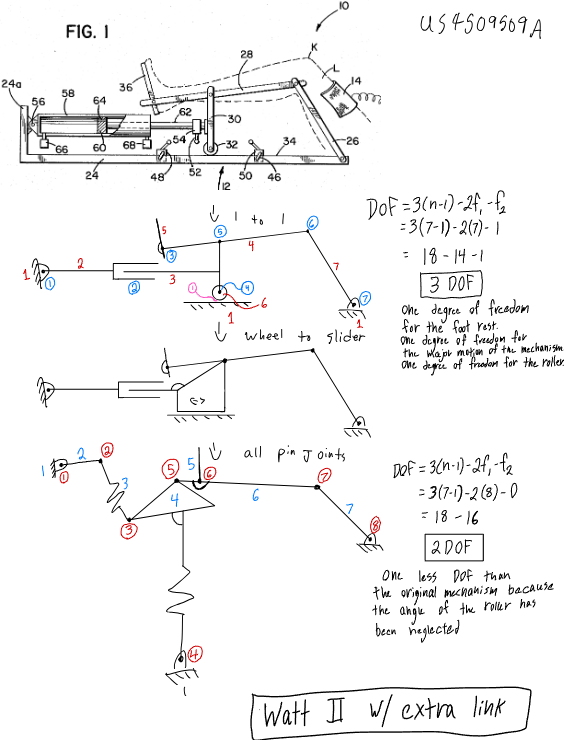
\includegraphics[width=0.54\linewidth]{../Kinematic Mechanism Images/4509509.png}
  \caption{Kinematics diagram for US4509509A apparatus.}
  \label{fig:US4509509A_kinematics}
\end{figure}

\subsection{Degrees of Freedom}
\[
\begin{aligned}
DOF &= 3(n-1) - 2f_1 - f_2 \\
DOF &= 3(7-1) - 2(8) - 0 \\
DOF &= 2
\end{aligned}
\]

The Mechanism, neglecting the roller position, has 2 degrees of freedom. One for the angle of the foot rest, and another for the main motion of the mechanism. The mechanism is a Watt II with an extra link.

\subsection{Observations}
This continuous passive motion (CPM) device highlights adjustability. The features include independent thigh and calf supports that are controlled by a motorized linkage. This mechanism consists of rotational joints providing reliable flexing and extending movements while maintaining a simple geometric relationship around limb segments. The design reflects a focus repeatable movement rather than anatomical precision. The ease of setup and durability also make it suitable for rehabilitation clinics. But the fixed-pivot nature of its motion path suggests limited ability to work with all of the ranges of motion of the human knee.

\subsection{Opportunities for Improvement}
Future iterations could enhance this design by introducing a virtual-pivot or cam-based linkage capable of replicating the knee's natural motion curve. This may improve patient comfort. Adjustment mechanisms and indexing certain stop points could simplify clinician setup and ensure more precise, repeatable motion ranges. The use of lightweight composites or hollow extrusions would also improve transportability and user comfort without sacrificing structural integrity.

\section{US4549534A: Leg Exercise Device}
\subsection{Description}
Continuous passive motion leg exerciser on an elongated base: thigh and lower-leg supports with a pivoting footplate ride on a sliding bearing, driven by a motorized threaded screw whose cycling reverses to produce repeatable knee bending.
\subsection{Images}
\begin{figure}[H]
  \centering
  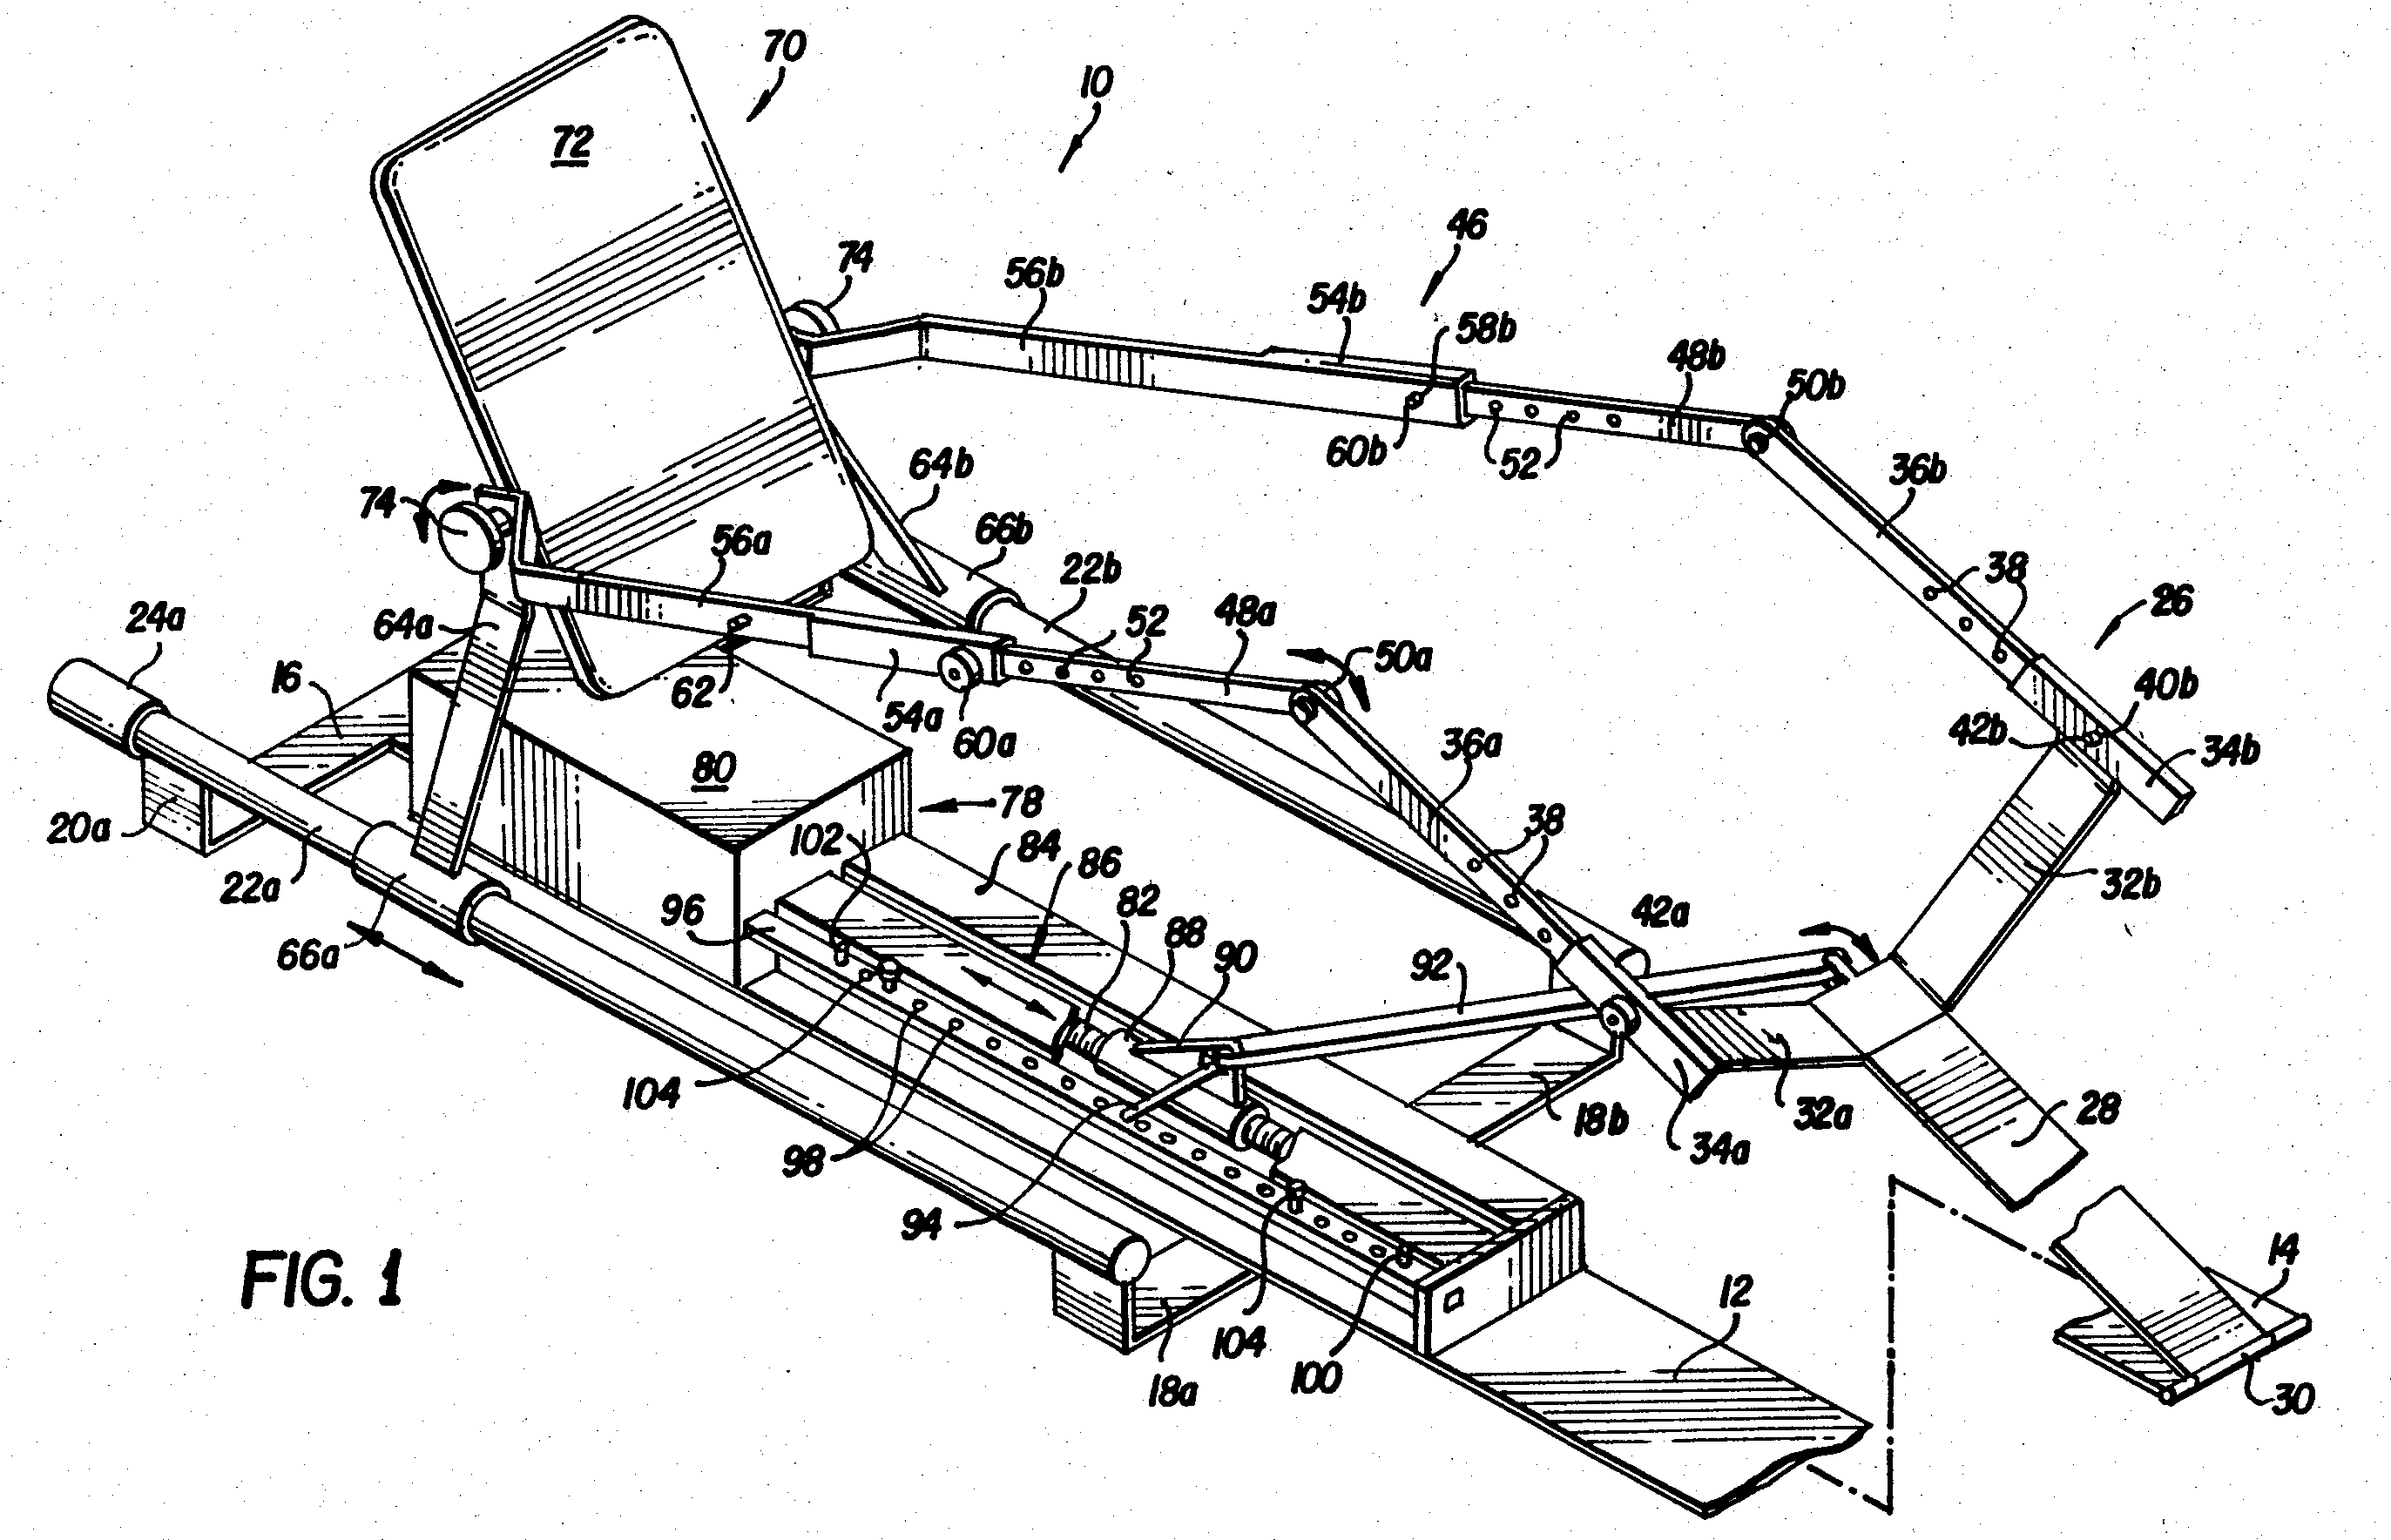
\includegraphics[width=0.54\linewidth]{US4549534.png}
  \caption{US4549534A leg exercise linkage aimed at repeatable passive motion.}
  \label{fig:US4549534A}
\end{figure}

\subsection{Mechanism kinematics}
\begin{figure}[H]
  \centering
  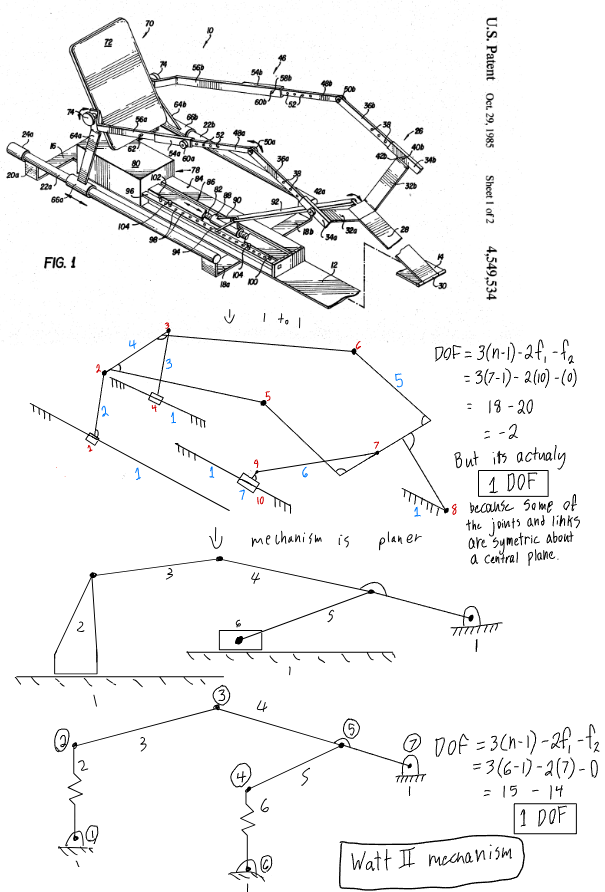
\includegraphics[width=0.54\linewidth]{../Kinematic Mechanism Images/4549534.png}
  \caption{Kinematics diagram for US4549534A leg exercise device.}
  \label{fig:US4549534A_kinematics}
\end{figure}

\subsection{Degrees of Freedom}
\[
\begin{aligned}
DOF &= 3(n-1) - 2f_1 - f_2 \\
DOF &= 3(6-1) - 2(7) - 0 \\
DOF &= 1
\end{aligned}
\]

The Mechanism has 1 degree of freedom and is a Watt II mechanism.

\subsection{Observations}
This design is accessible and compact, offering an easy use mechanical structure intended for home rehabilitation. The device uses a single pivot or short-link mechanism that supports the lower leg and guides it through a prescribed flexion/extension path. The simplicity minimizes cost and setup time, but it also limits the range of motion adjustments. This could potentially lead to suboptimal alignment for users with different leg lengths or limb sizes. Ultimately this design trades accessibility for patient specific needs.

\subsection{Opportunities for Improvement}
Enhancing adjustability would significantly improve the functionality of this mechanism. Sliding pivots or telescoping linkages could help align the mechanical axis more closely with the user's knee joint, reducing discomfort and improving therapeutic effectiveness. Soft, interchangeable limb supports could further increase comfort and accommodate different patient anatomies.

\section{US4566440A: Orthosis for Leg Movement with Virtual Hip Pivot}
\subsection{Description}
Leg exercise orthosis using a double four-bar linkage to create a virtual hip pivot while guiding femur and tibia supports, enabling coordinated hip–knee–ankle motion with improved anatomical alignment.
\subsection{Images}
\begin{figure}[H]
  \centering
  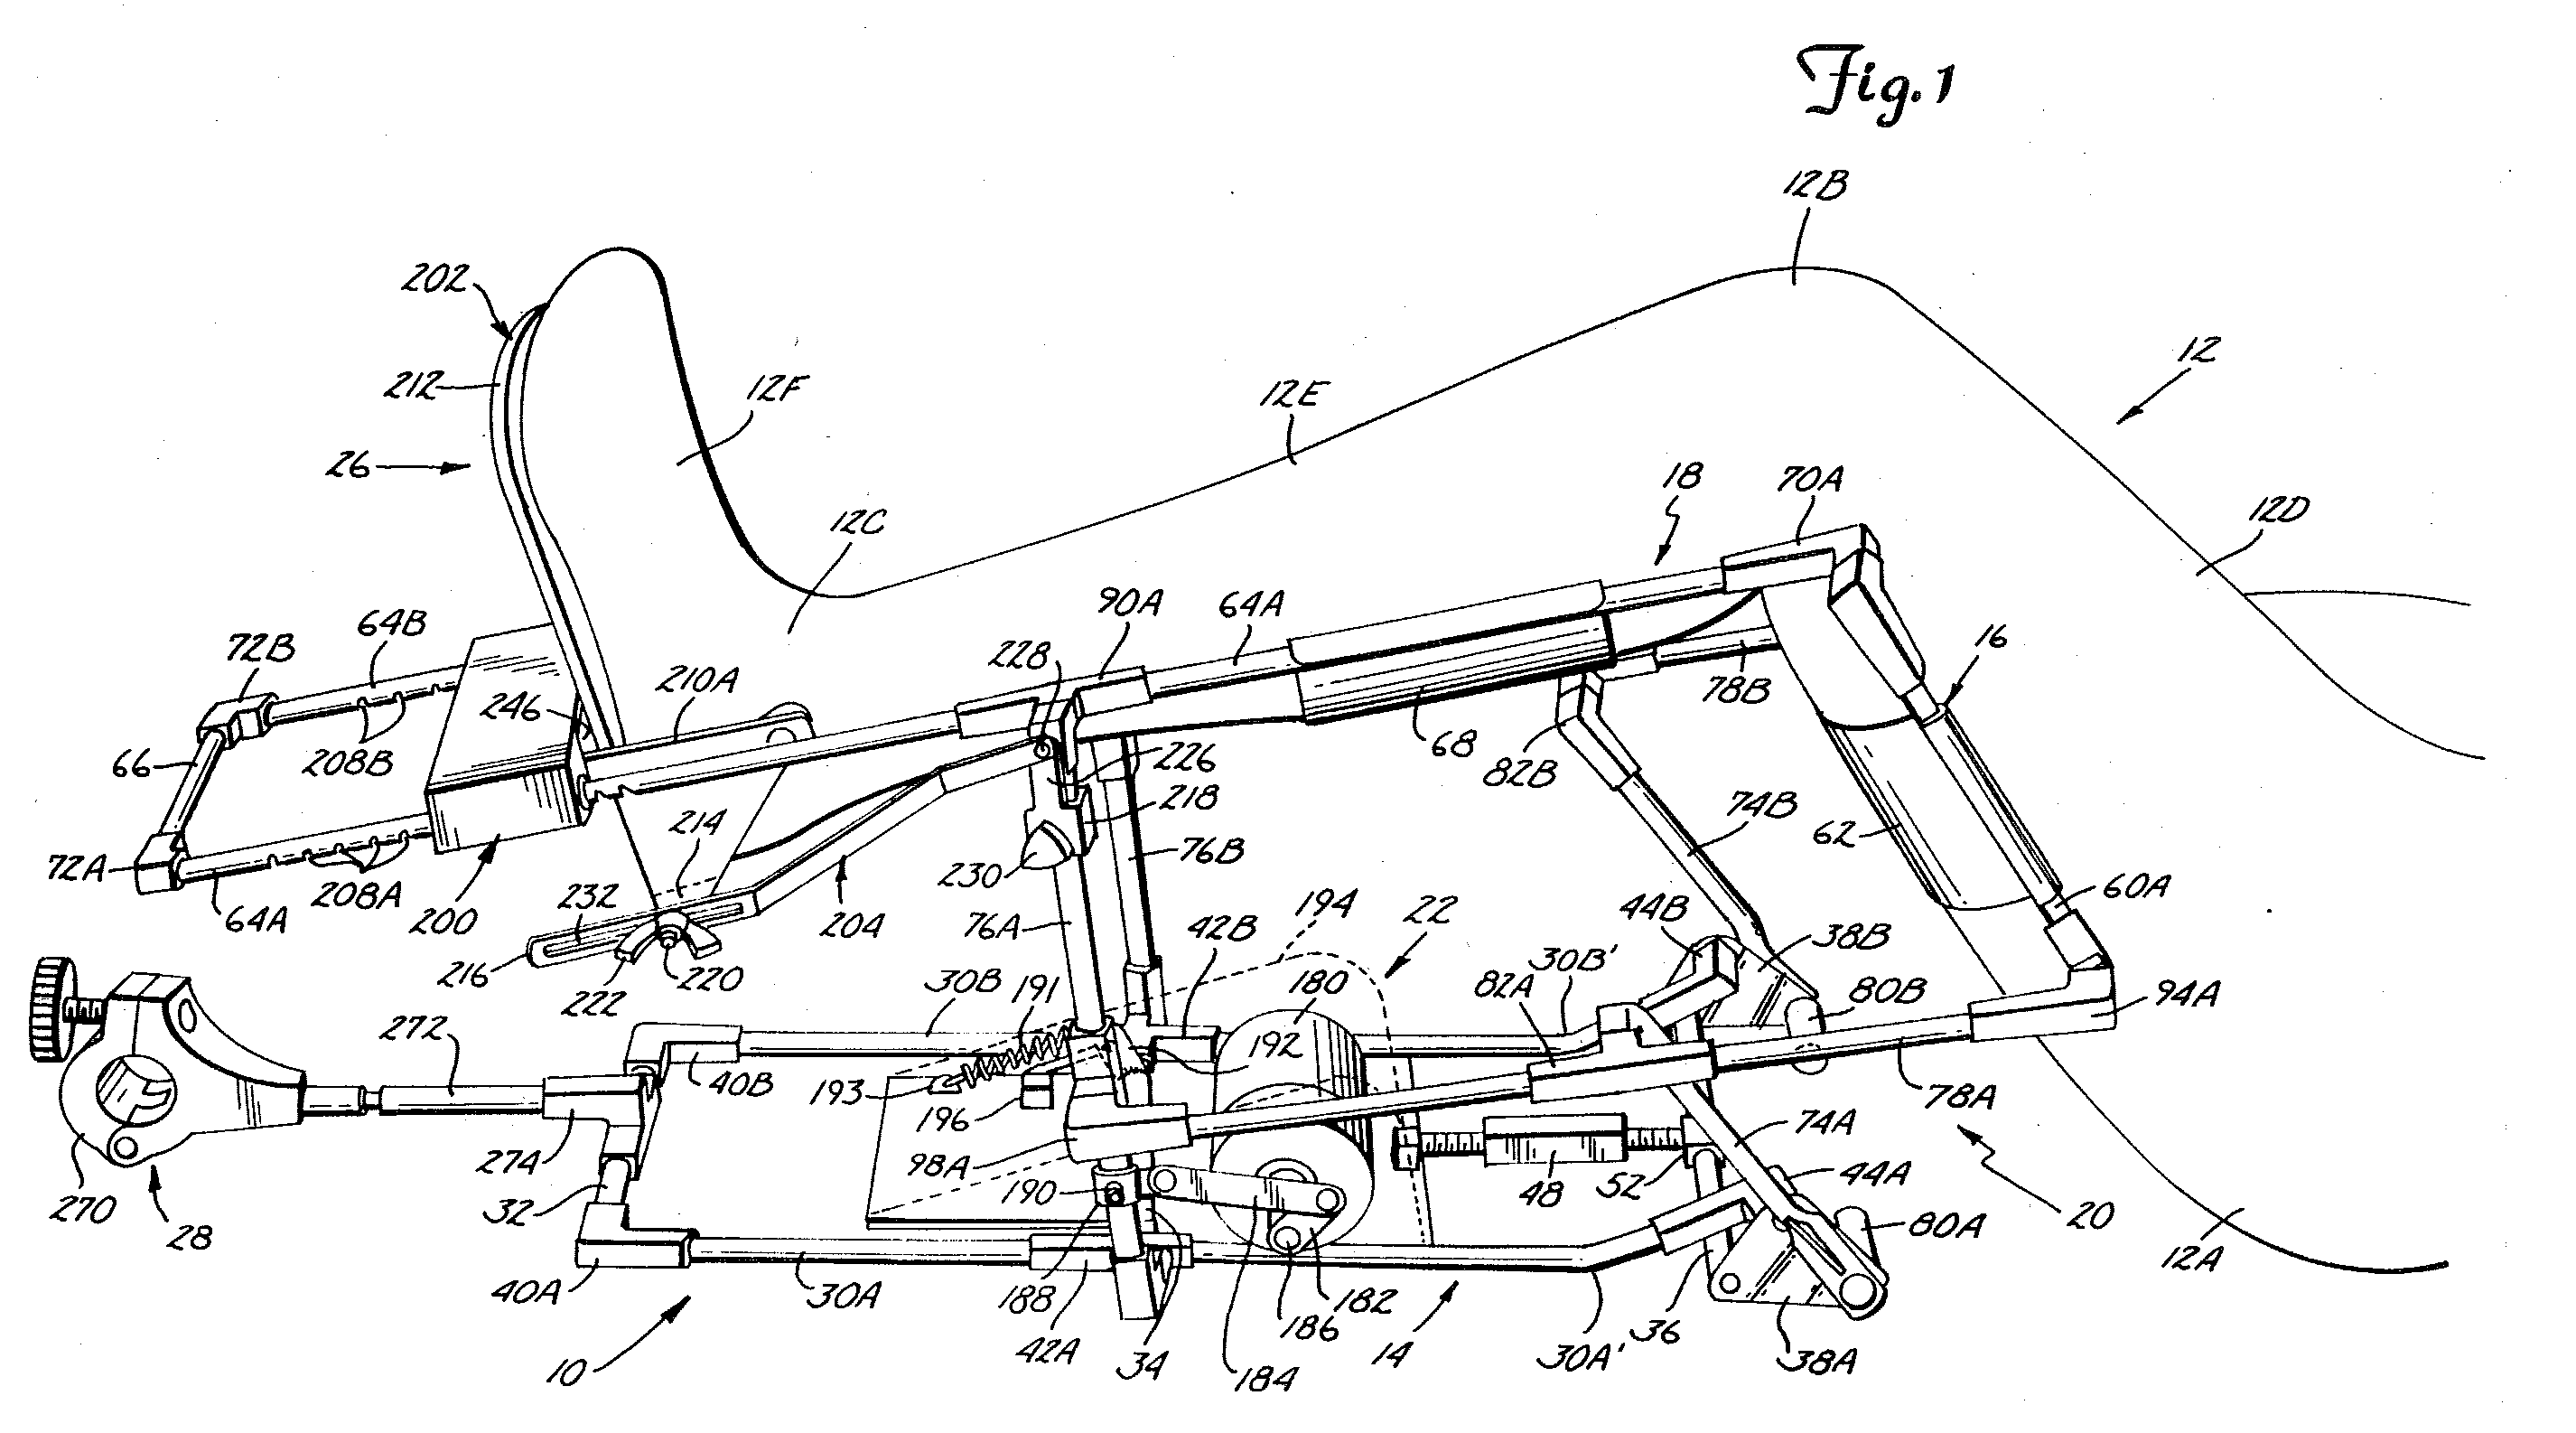
\includegraphics[width=0.54\linewidth]{US4566440_1.png}
  \caption{US4566440A orthosis showing geometry for a virtual hip pivot.}
  \label{fig:US4566440A}
\end{figure}

\subsection{Mechanism kinematics}
\begin{figure}[H]
  \centering
  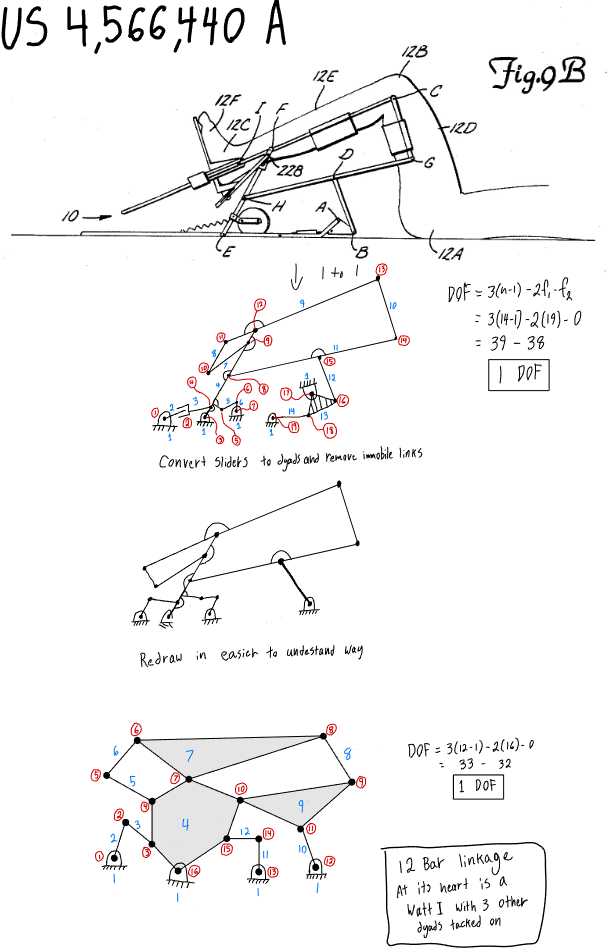
\includegraphics[width=0.54\linewidth]{../Kinematic Mechanism Images/4566440.png}
  \caption{Kinematics diagram for US4566440A orthosis with virtual hip pivot.}
  \label{fig:US4566440A_kinematics}
\end{figure}

\subsection{Degrees of Freedom}
\[
\begin{aligned}
DOF &= 3(n-1) - 2f_1 - f_2 \\
DOF &= 3(12-1) - 2(16) - 0 \\
DOF &= 1
\end{aligned}
\]

The Mechanism has 1 degree of freedom and is a Watt I mechanism with several dyads added.

\subsection{Observations}
This patent represents a very anatomically accurate design by introducing a virtual-pivot mechanism to replicate natural hip motion during lower-limb rehabilitation. Unlike fixed-pivot orthoses, the multi-link arrangement in this design creates an instantaneous center of rotation that migrates during motion, better matching the body's kinematics. The system demonstrates an understanding of motion synthesis and human biomechanics, achieving greater comfort and reduced shear compared to simpler linkages. The complexity of the linkages will only hinder this product for manufacturing costs.

\subsection{Opportunities for Improvement}
The primary improvements would involve simplifying the geometry while retaining the axis following behavior. Type synthesis techniques could identify an equivalent four bar configuration that reduces parts without sacrificing motion accuracy. Adjustable geometry settings or quick calibration mechanisms could allow clinicians to tailor the virtual-pivot path to individual patients. These refinements would improve manufacturability, reduce weight, and streamline clinical setup, enhancing both performance and practicality.

\section{US4974830A: Continuous Passive Motion Device}
\subsection{Description}
CPM device with a single cantilevered drive tube supporting calf and thigh drive bars; adjustable cradles on rotatable arms permit use on either leg, with a cantilevered foot support and a bed-end mount incorporating rack-and-pinion plus gas spring assist for lifting/rotation.
\subsection{Images}
\begin{figure}[H]
  \centering
  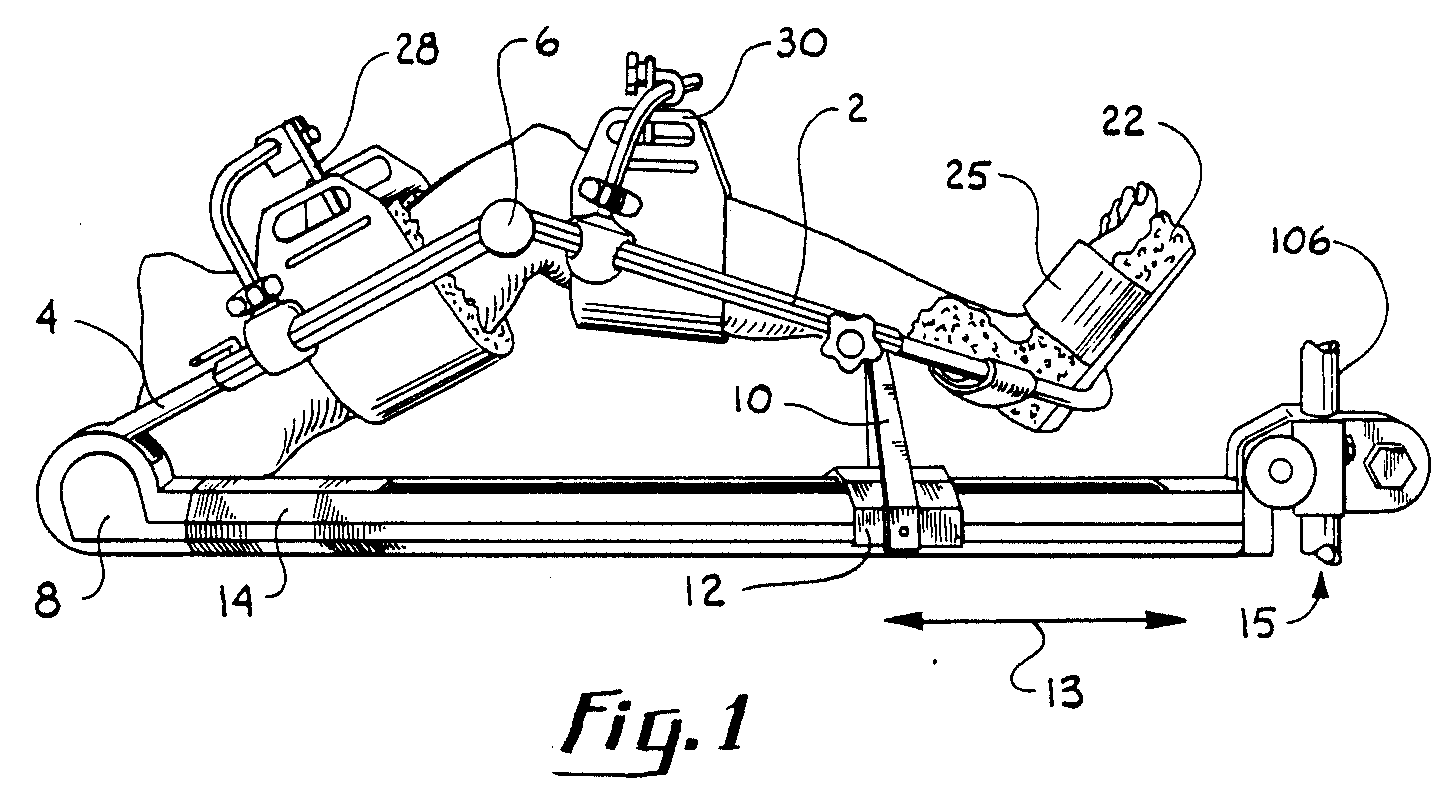
\includegraphics[width=0.54\linewidth]{US4974830_1.png}
  \caption{US4974830A CPM with adjustable cradles and end-stop control.}
  \label{fig:US4974830A}
\end{figure}

\subsection{Mechanism kinematics}
\begin{figure}[H]
  \centering
  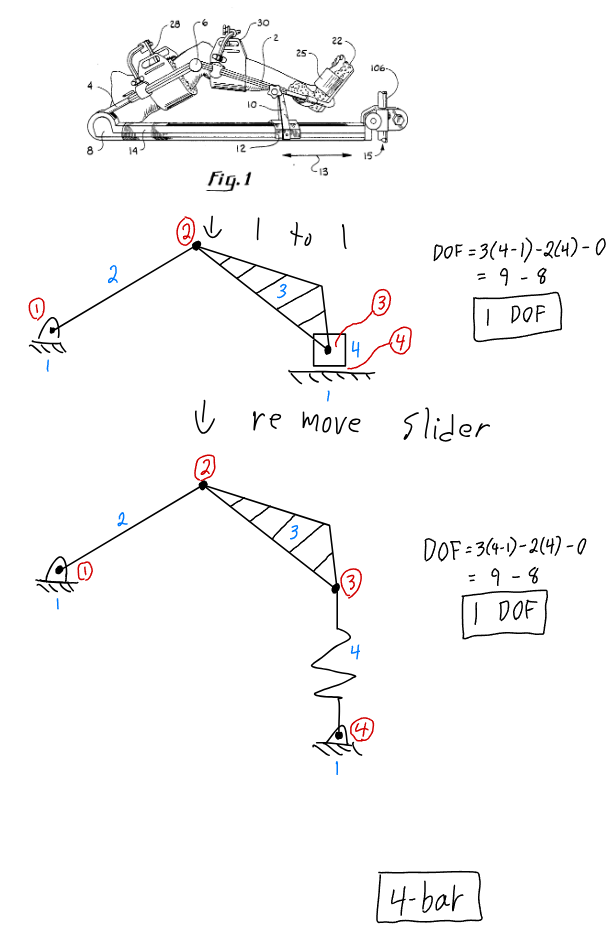
\includegraphics[width=0.54\linewidth]{../Kinematic Mechanism Images/4974830.png}
  \caption{Kinematics diagram for US4974830A continuous passive motion device.}
  \label{fig:US4974830A_kinematics}
\end{figure}

\subsection{Degrees of Freedom}
\[
\begin{aligned}
DOF &= 3(n-1) - 2f_1 - f_2 \\
DOF &= 3(4-1) - 2(4) - 0 \\
DOF &= 1
\end{aligned}
\]

The mechanism simplified to a 4 bar linkage with 1 degree of freedom.

\subsection{Observations}
This patent involves programmable control in the range of motion and repetition cycles, which highlights patient adjustability in those two ways. This mechanism maintains a conventional linkage architecture while also integrating motorized actuation and digital interface elements that are adjustable to clinicians or other users. While this configuration enhances repeatability and safety, the mechanical design remains relatively bulky and dependent on manual adjustment of limb supports.

\subsection{Opportunities for Improvement}
Future advancements could replace mechanical end stops with electronic soft limits coupled to torque sensors, allowing the system to detect patient resistance and automatically modulate motion for safety and comfort. Incorporating a user-friendly interface with preprogrammed therapy profiles would simplify setup and reduce clinician workload. Additionally, a modular design using lightweight materials could make the unit more portable and suitable for both clinical and home settings. These refinements would bring the design in line with modern ergonomic and usability standards while maintaining the programmability that defines its innovation.

\section{US5333604A: Patella Exercising Apparatus}
\subsection{Description}
Patella exercise attachment for a CPM device employing a patella contact pad that biases the patella superiorly or inferiorly during flexion/extension; a spring-like cam sets force to mobilize tracking and help prevent patella baja.
\subsection{Images}
\begin{figure}[H]
  \centering
  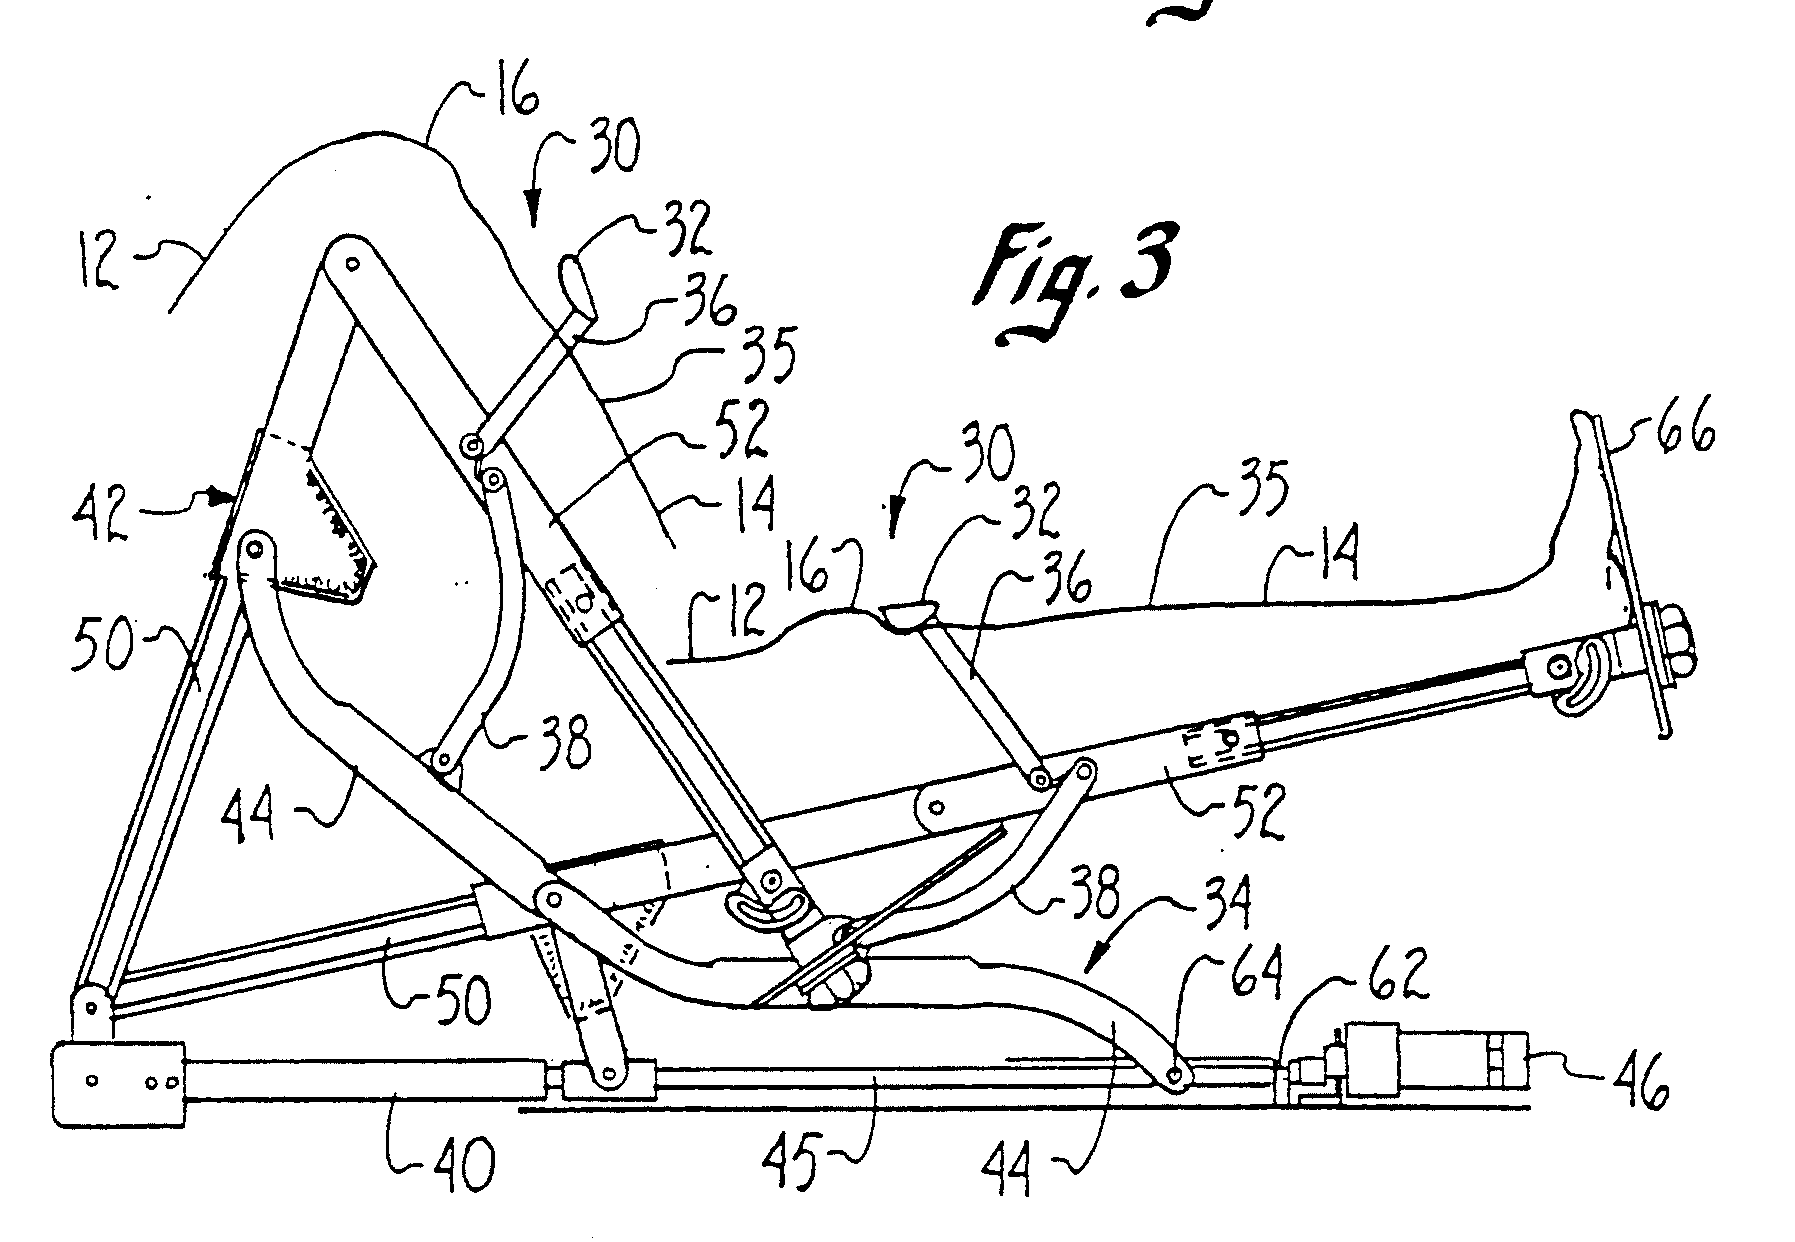
\includegraphics[width=0.54\linewidth]{US5333604_1.png}
  \caption{US5333604A apparatus for targeted patellar motion and tracking.}
  \label{fig:US5333604A}
\end{figure}

\subsection{Mechanism kinematics}
\begin{figure}[H]
  \centering
  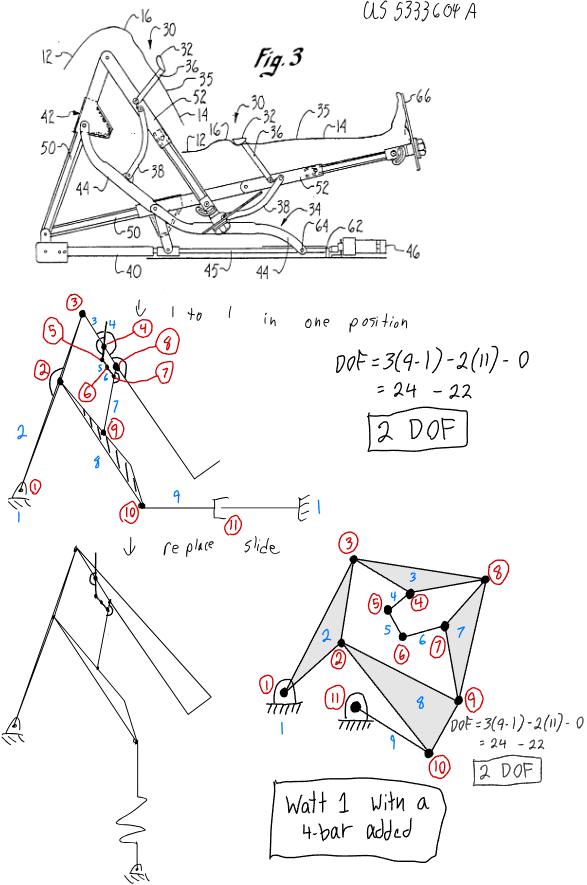
\includegraphics[width=0.54\linewidth]{../Kinematic Mechanism Images/5333604.png}
  \caption{Kinematics diagram for US5333604A patella exercising apparatus.}
  \label{fig:US5333604A_kinematics}
\end{figure}

\subsection{Degrees of Freedom}
\[
\begin{aligned}
DOF &= 3(n-1) - 2f_1 - f_2 \\
DOF &= 3(9-1) - 2(11) - 0 \\
DOF &= 2
\end{aligned}
\]

The mechanism has 2 degrees of freedom and is a Watt II mechanism with an added 4 bar linkage.

\subsection{Observations}
This device focuses on isolated patellar movement to address patellofemoral disorders that other CPM devices ignore. It uses guided track or small linkage that translates and tilts the patella within a controlled range. This mechanical isolation shows a targeted approach to improving tracking and reducing joint pain. As a standalone device it is limited and needs to be used in cooperation with other devices to have full healing of the targeted area.

\subsection{Opportunities for Improvement}
Incorporating interfaces that emulate the soft-tissue environment could improve comfort and better approximate physiological movement. Adjustable resistance could further customize therapy for different patient needs. These improvements would transform a niche design into a versatile, complementary tool within comprehensive knee rehabilitation systems.

\section{US6267735B1: Continuous Passive Motion Device Having a Comfort Zone Feature}
\subsection{Description}
Therapeutic CPM with a ``Comfort Zone'' range-of-motion feature that temporarily increases flexion (or decreases extension) to alleviate discomfort, then automatically returns toward preset ROM limits over time; includes controlled deceleration near limits and smooth acceleration away from them.
\subsection{Images}
\begin{figure}[H]
  \centering
  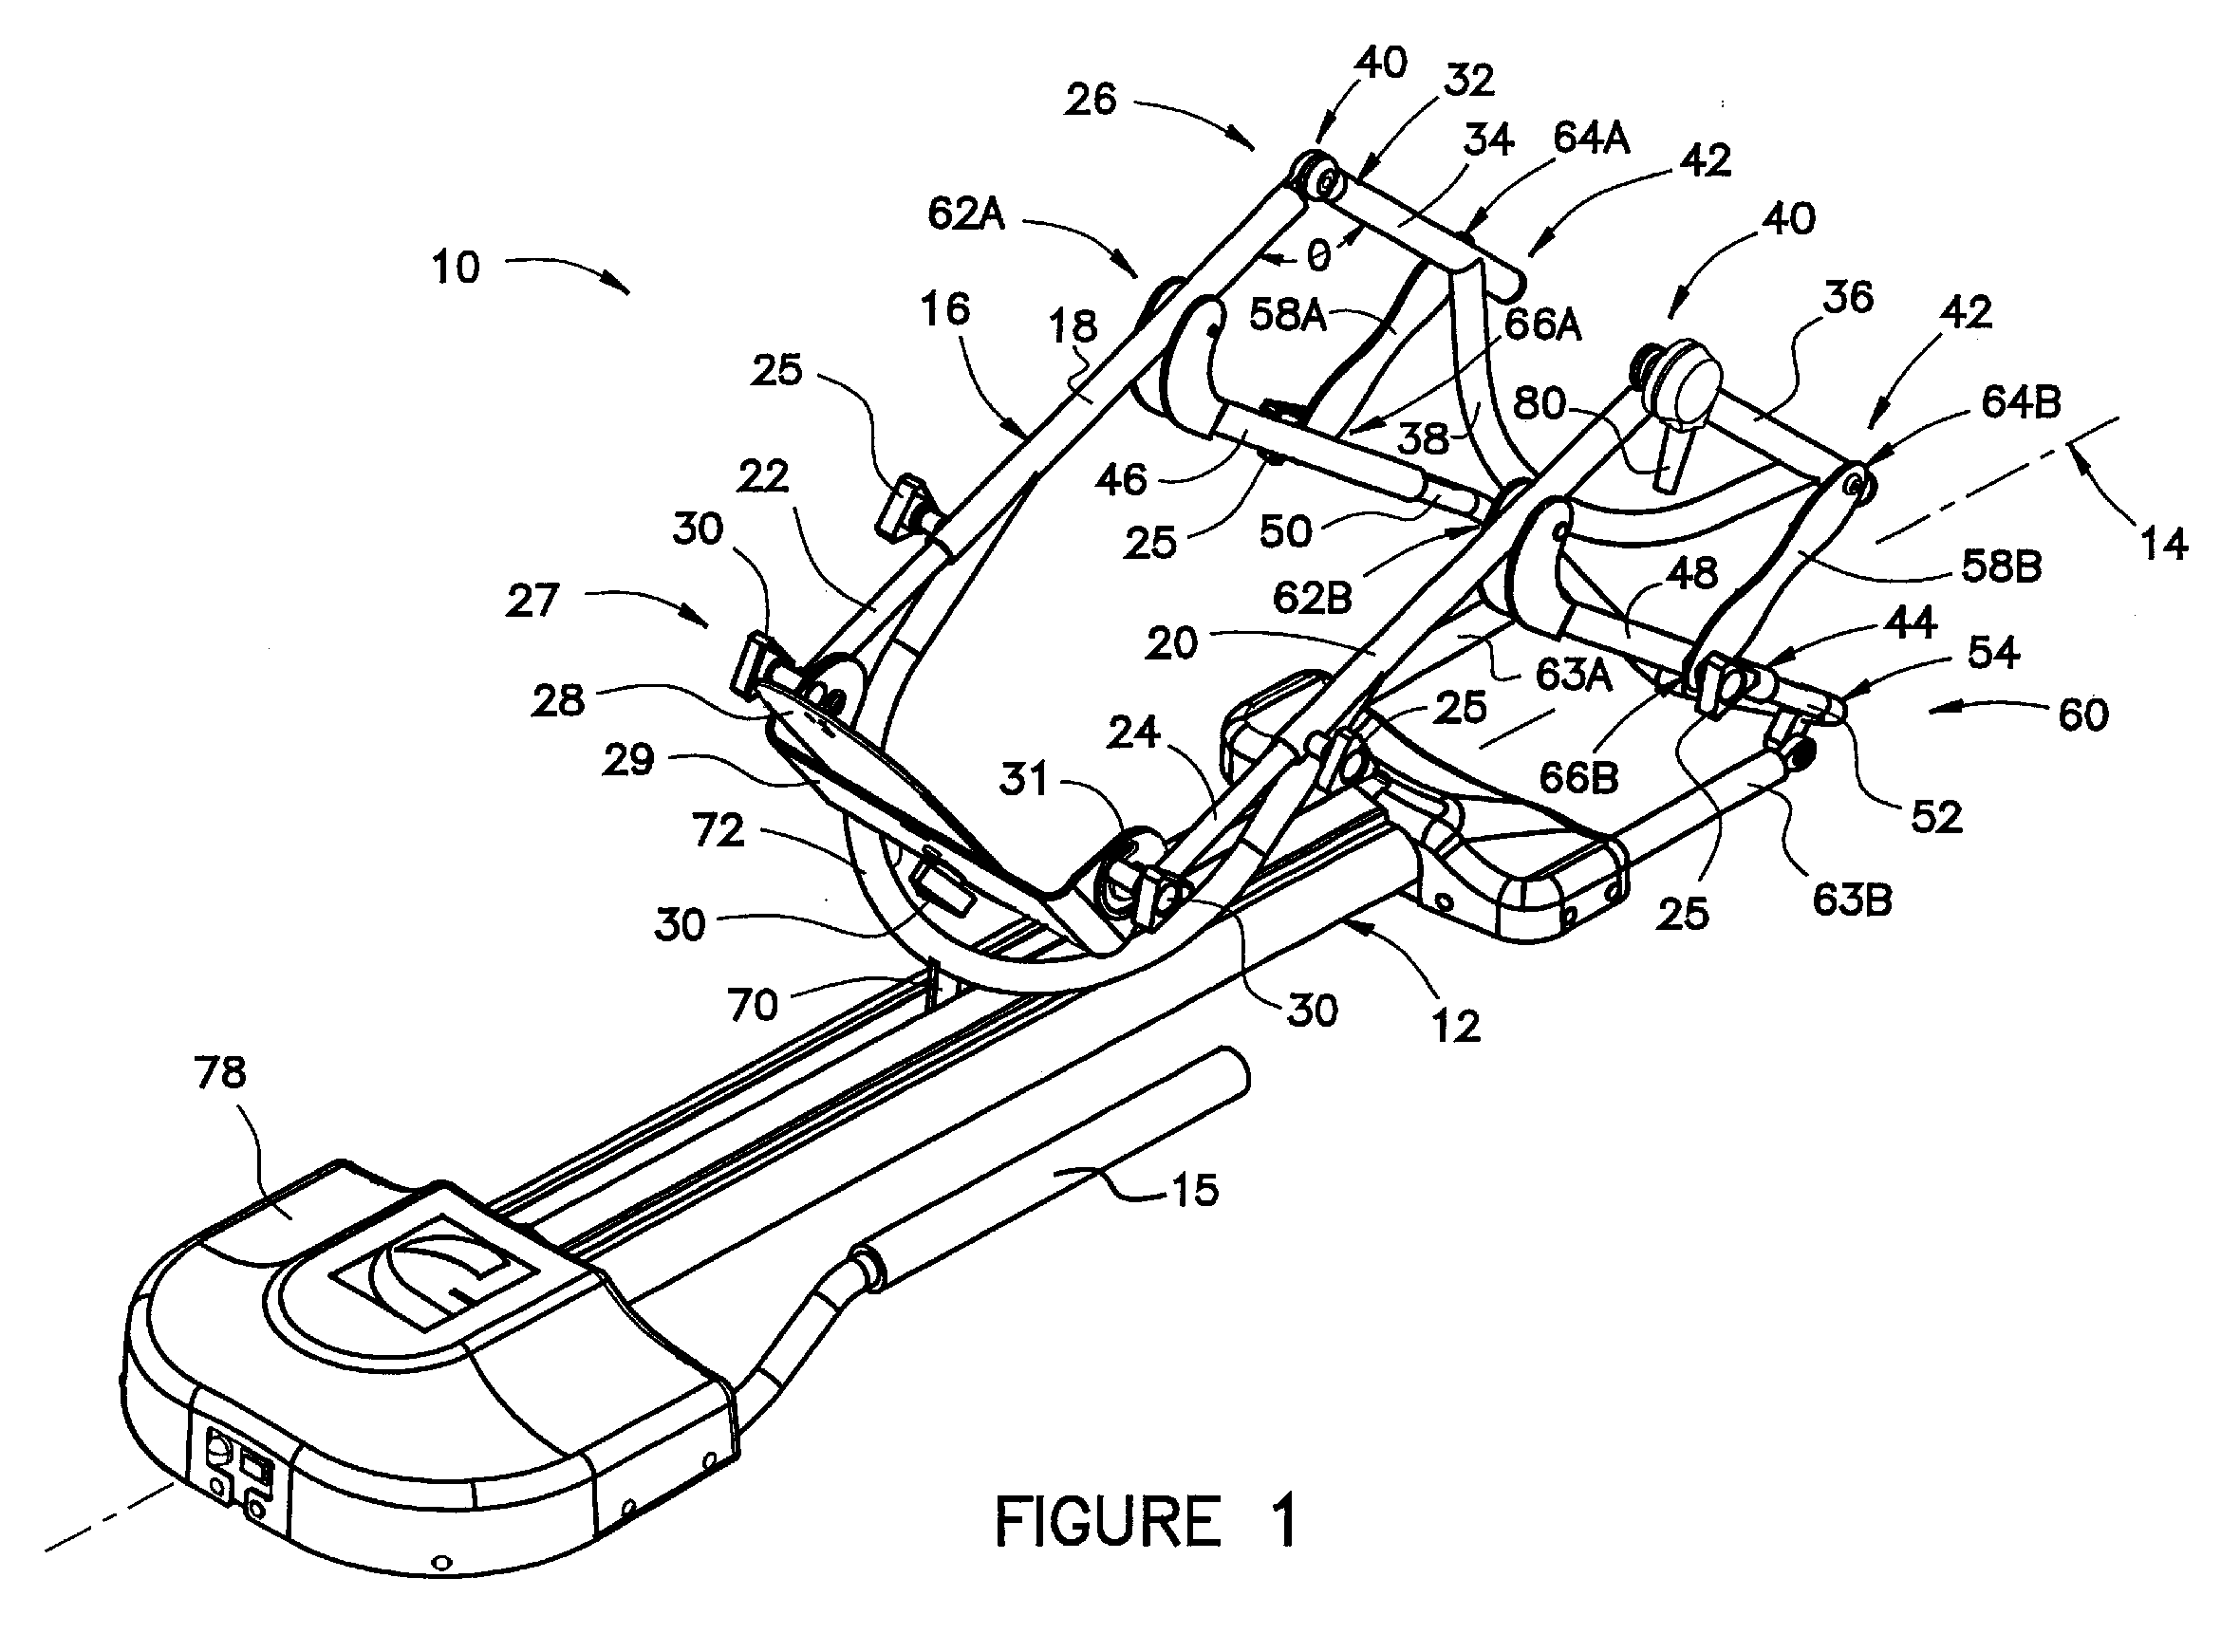
\includegraphics[width=0.54\linewidth]{US6267735B1_1.png}
  \caption{US6267735B1 CPM featuring an adaptive comfort-zone deadband.}
  \label{fig:US6267735B1}
\end{figure}

\subsection{Mechanism kinematics}
\begin{figure}[H]
  \centering
  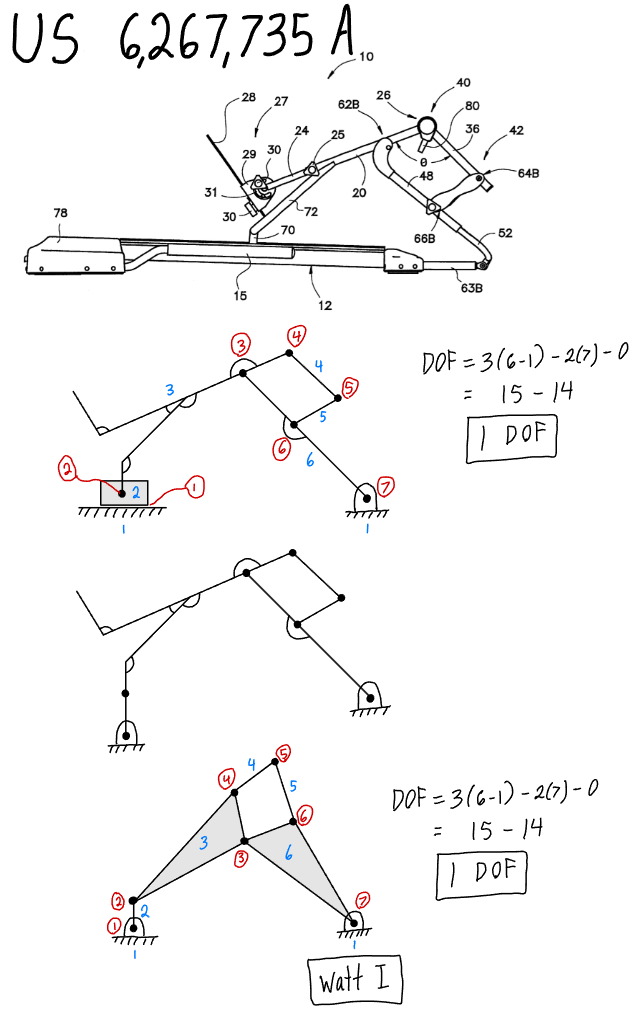
\includegraphics[width=0.54\linewidth]{../Kinematic Mechanism Images/6267735.png}
  \caption{Kinematics diagram for US6267735B1 CPM device with comfort zone feature.}
  \label{fig:US6267735B1_kinematics}
\end{figure}

\subsection{Degrees of Freedom}
\[
\begin{aligned}
DOF &= 3(n-1) - 2f_1 - f_2 \\
DOF &= 3(6-1) - 2(7) - 0 \\
DOF &= 1
\end{aligned}
\]

The mechanism has 1 degree of freedom and is a Watt I mechanism.

\subsection{Observations}
This patent has an ergonomic improvement through a "comfort zone" feature. This is an adaptive control system that automatically adjusts motion speed or reverses direction before reaching painful joint limits. By focusing on reducing pain induced muscle guarding, this design enhances compliance and overall rehabilitation outcomes. The control system's sophistication may increase complexity and maintenance requirements compared to simpler mechanical designs.

\subsection{Opportunities for Improvement}
To further enhance this product development could involve patient specific calibration modes that learn and adapt comfort thresholds over time. This could potentially provide more personalized therapy. Integrating torque and motion sensors with a digital feedback interface would enable real-time monitoring of patient responses. Smooth acceleration and deceleration algorithms could further refine comfort and safety. These improvements would transform the concept from a reactive control system into an intelligent, adaptive therapeutic platform that anticipates and responds to user feedback dynamically.

\section{US6325770B1: Device for Producing Continuous Passive Motion}
\subsection{Description}
Device for producing CPM with a reciprocating driving element on a base; upper and lower limb supports pivot about a transverse axis. A linking element pivotally connects the upper support to the driver, while the lower support slides against the link to generate the bending/extension cycle.
\subsection{Images}
\begin{figure}[H]
  \centering
  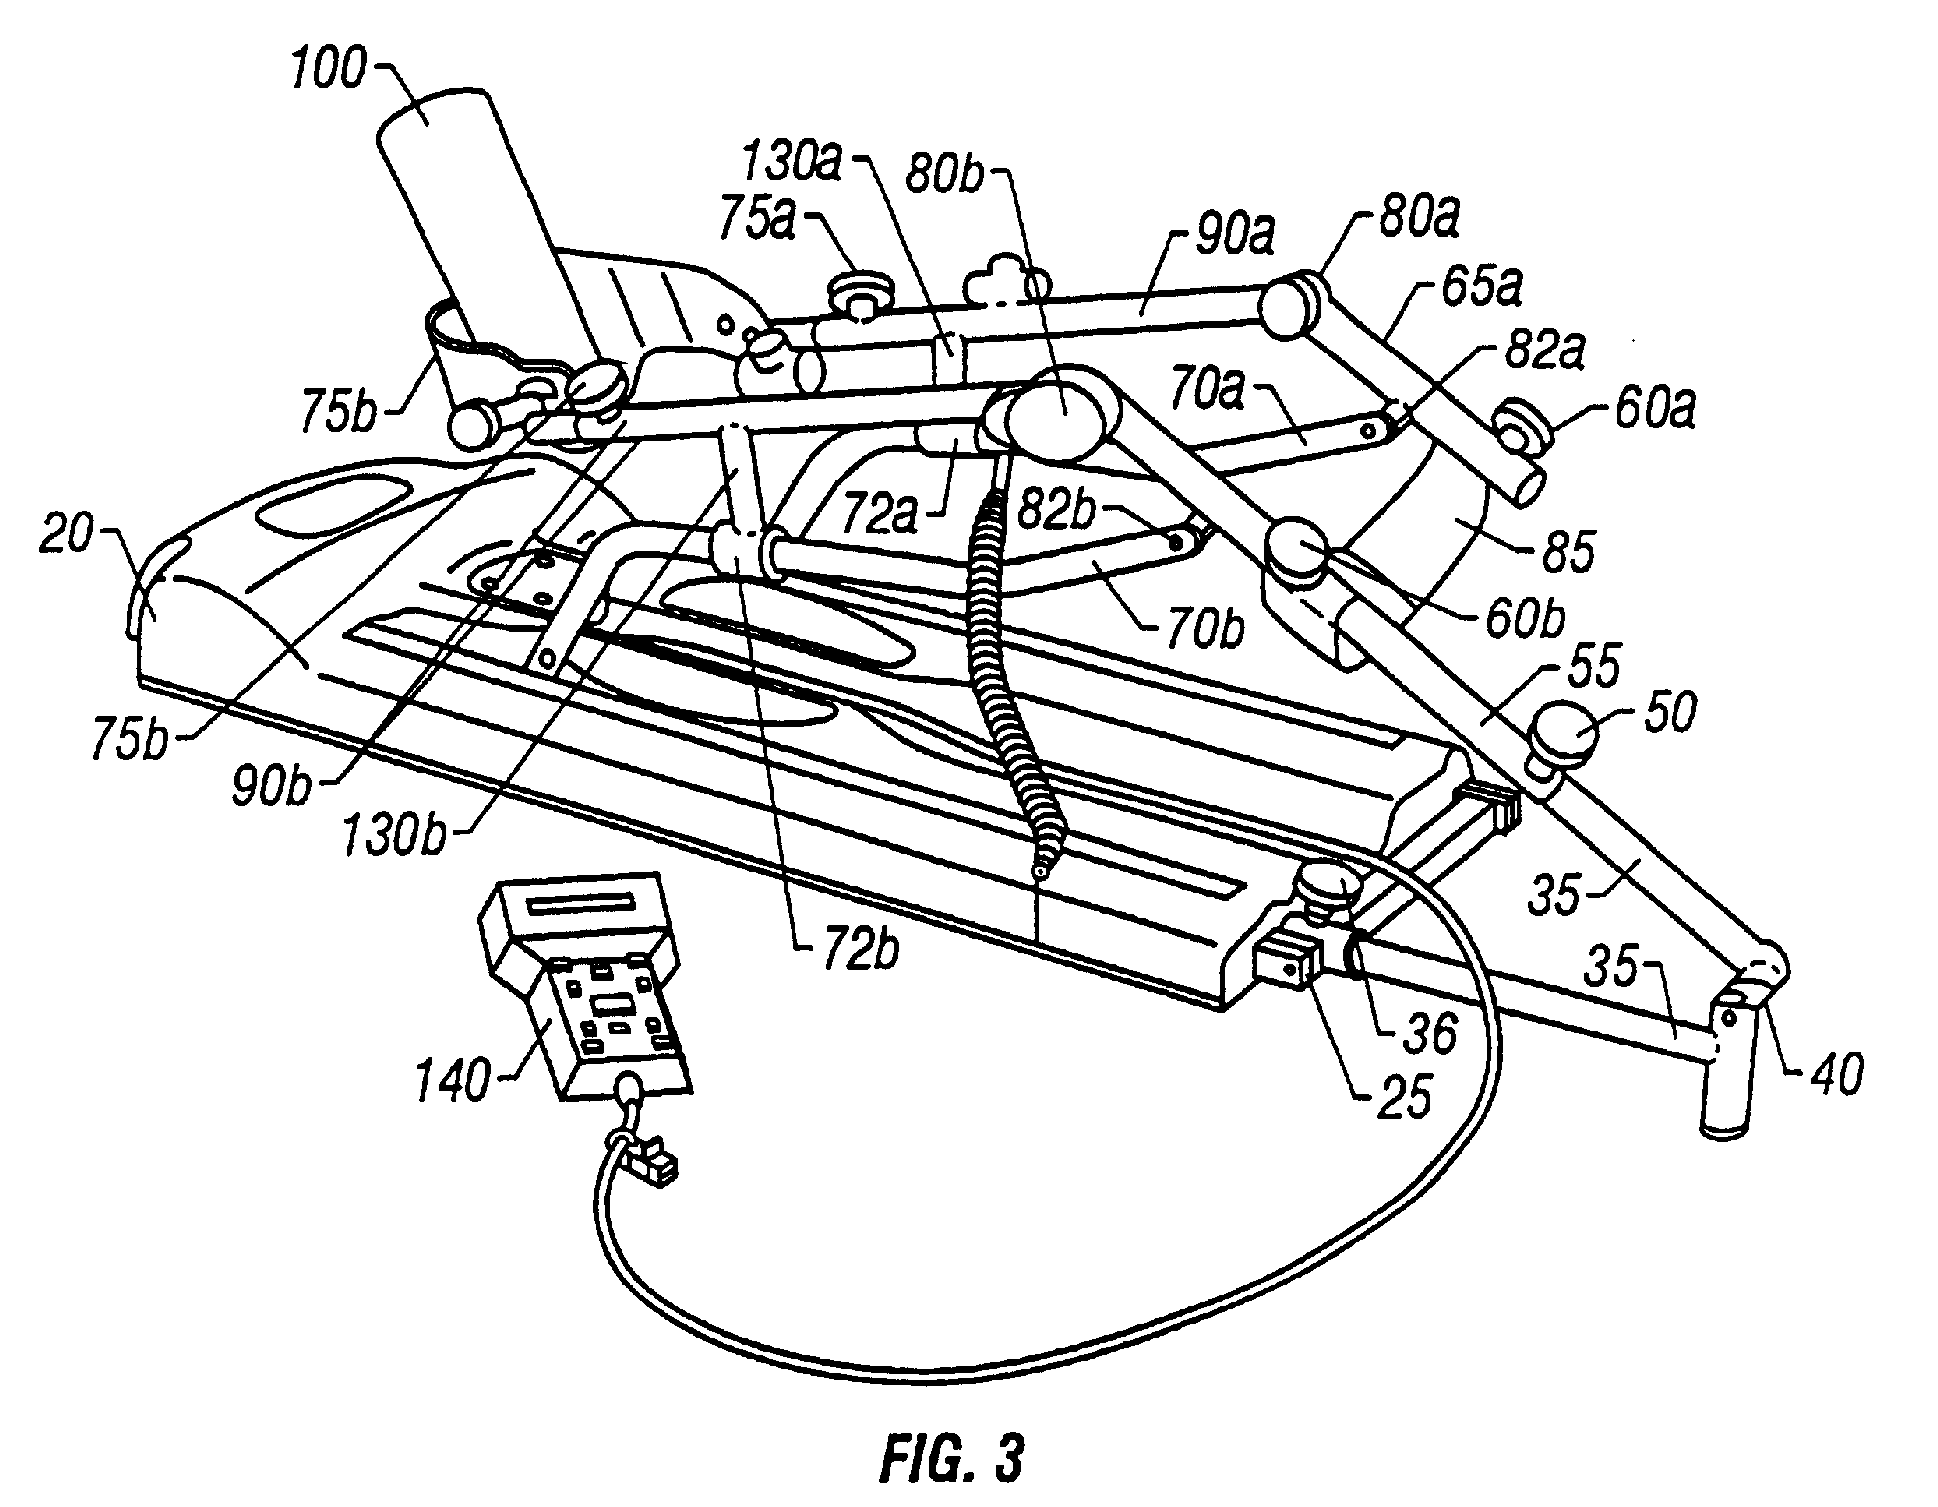
\includegraphics[width=0.54\linewidth]{US6325770B1_1.png}
  \caption{US6325770B1 transmission tuned for knee-like motion paths.}
  \label{fig:US6325770B1}
\end{figure}

\subsection{Mechanism kinematics}
\begin{figure}[H]
  \centering
  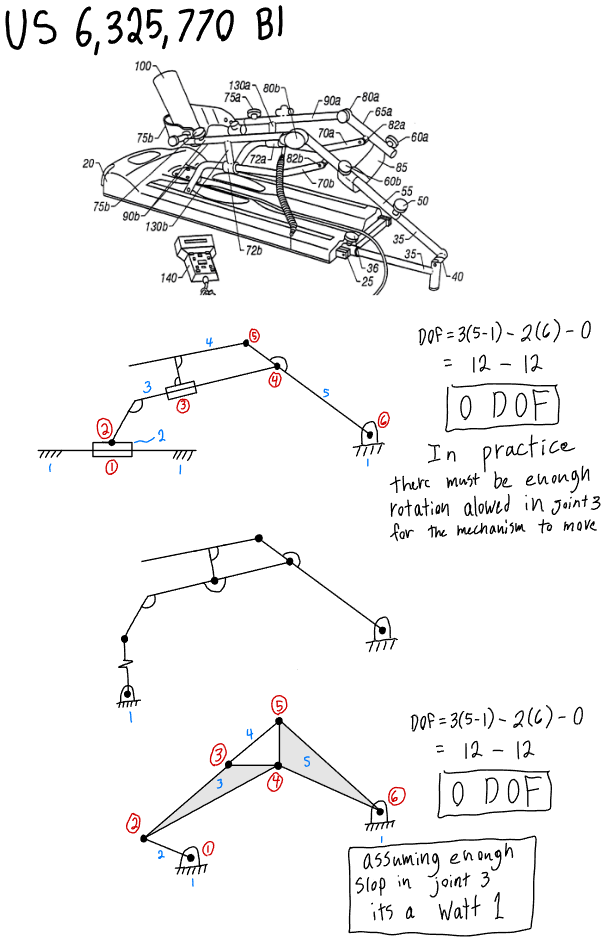
\includegraphics[width=0.54\linewidth]{../Kinematic Mechanism Images/6325770.png}
  \caption{Kinematics diagram for US6325770B1 device for producing continuous passive motion.}
  \label{fig:US6325770B1_kinematics}
\end{figure}

\subsection{Degrees of Freedom}
\[
\begin{aligned}
DOF &= 3(n-1) - 2f_1 - f_2 \\
DOF &= 3(5-1) - 2(6) - 0 \\
DOF &= 0
\end{aligned}
\]

The mechanism has 0 degrees of freedom according to our analysis, though there may be details missing from the drawing. We assume there must be rotation at joint 3 to allow mechanism 1 degree of freedom.

\subsection{Observations}
This design uses cam and gear transmissions to generate a motion profile that better mimics the natural kinematics of the knee joint. Unlike traditional rotary or linear drives, the cam mechanism allows nonuniform angular velocity and displacement, producing a smoother, more physiologically accurate movement. The use of tuned cams also helps reduce mechanical backlash and improve motion precision. The fixed cam geometry may limit adaptability across patients with different anatomical characteristics or therapeutic requirements.

\subsection{Opportunities for Improvement}
One promising enhancement would be the implementation of interchangeable or adjustable cam profiles to accommodate varying knee geometries and rehabilitation goals. Incorporating modern materials and precision machining could reduce weight and wear while maintaining the smooth motion advantage. Additionally, compliant joints or flexible couplings could be integrated to absorb small misalignments, minimizing shear at the patient interface. Together, these refinements would maintain the benefits of the cam-driven approach while improving adaptability and patient-specific performance.

\section{US5252102A: Electronic Range of Motion Apparatus for Orthosis/Prosthesis/CPM}
\subsection{Description}
Electronic ROM apparatus with a remote subsystem that sends motion commands to a local controller on an orthosis, prosthesis, or CPM device. The local controller governs actuator position, speed, and direction; stopping positions are programmable and selectable, with sleep mode when idle to conserve power.
\subsection{Images}
\begin{figure}[H]
  \centering
  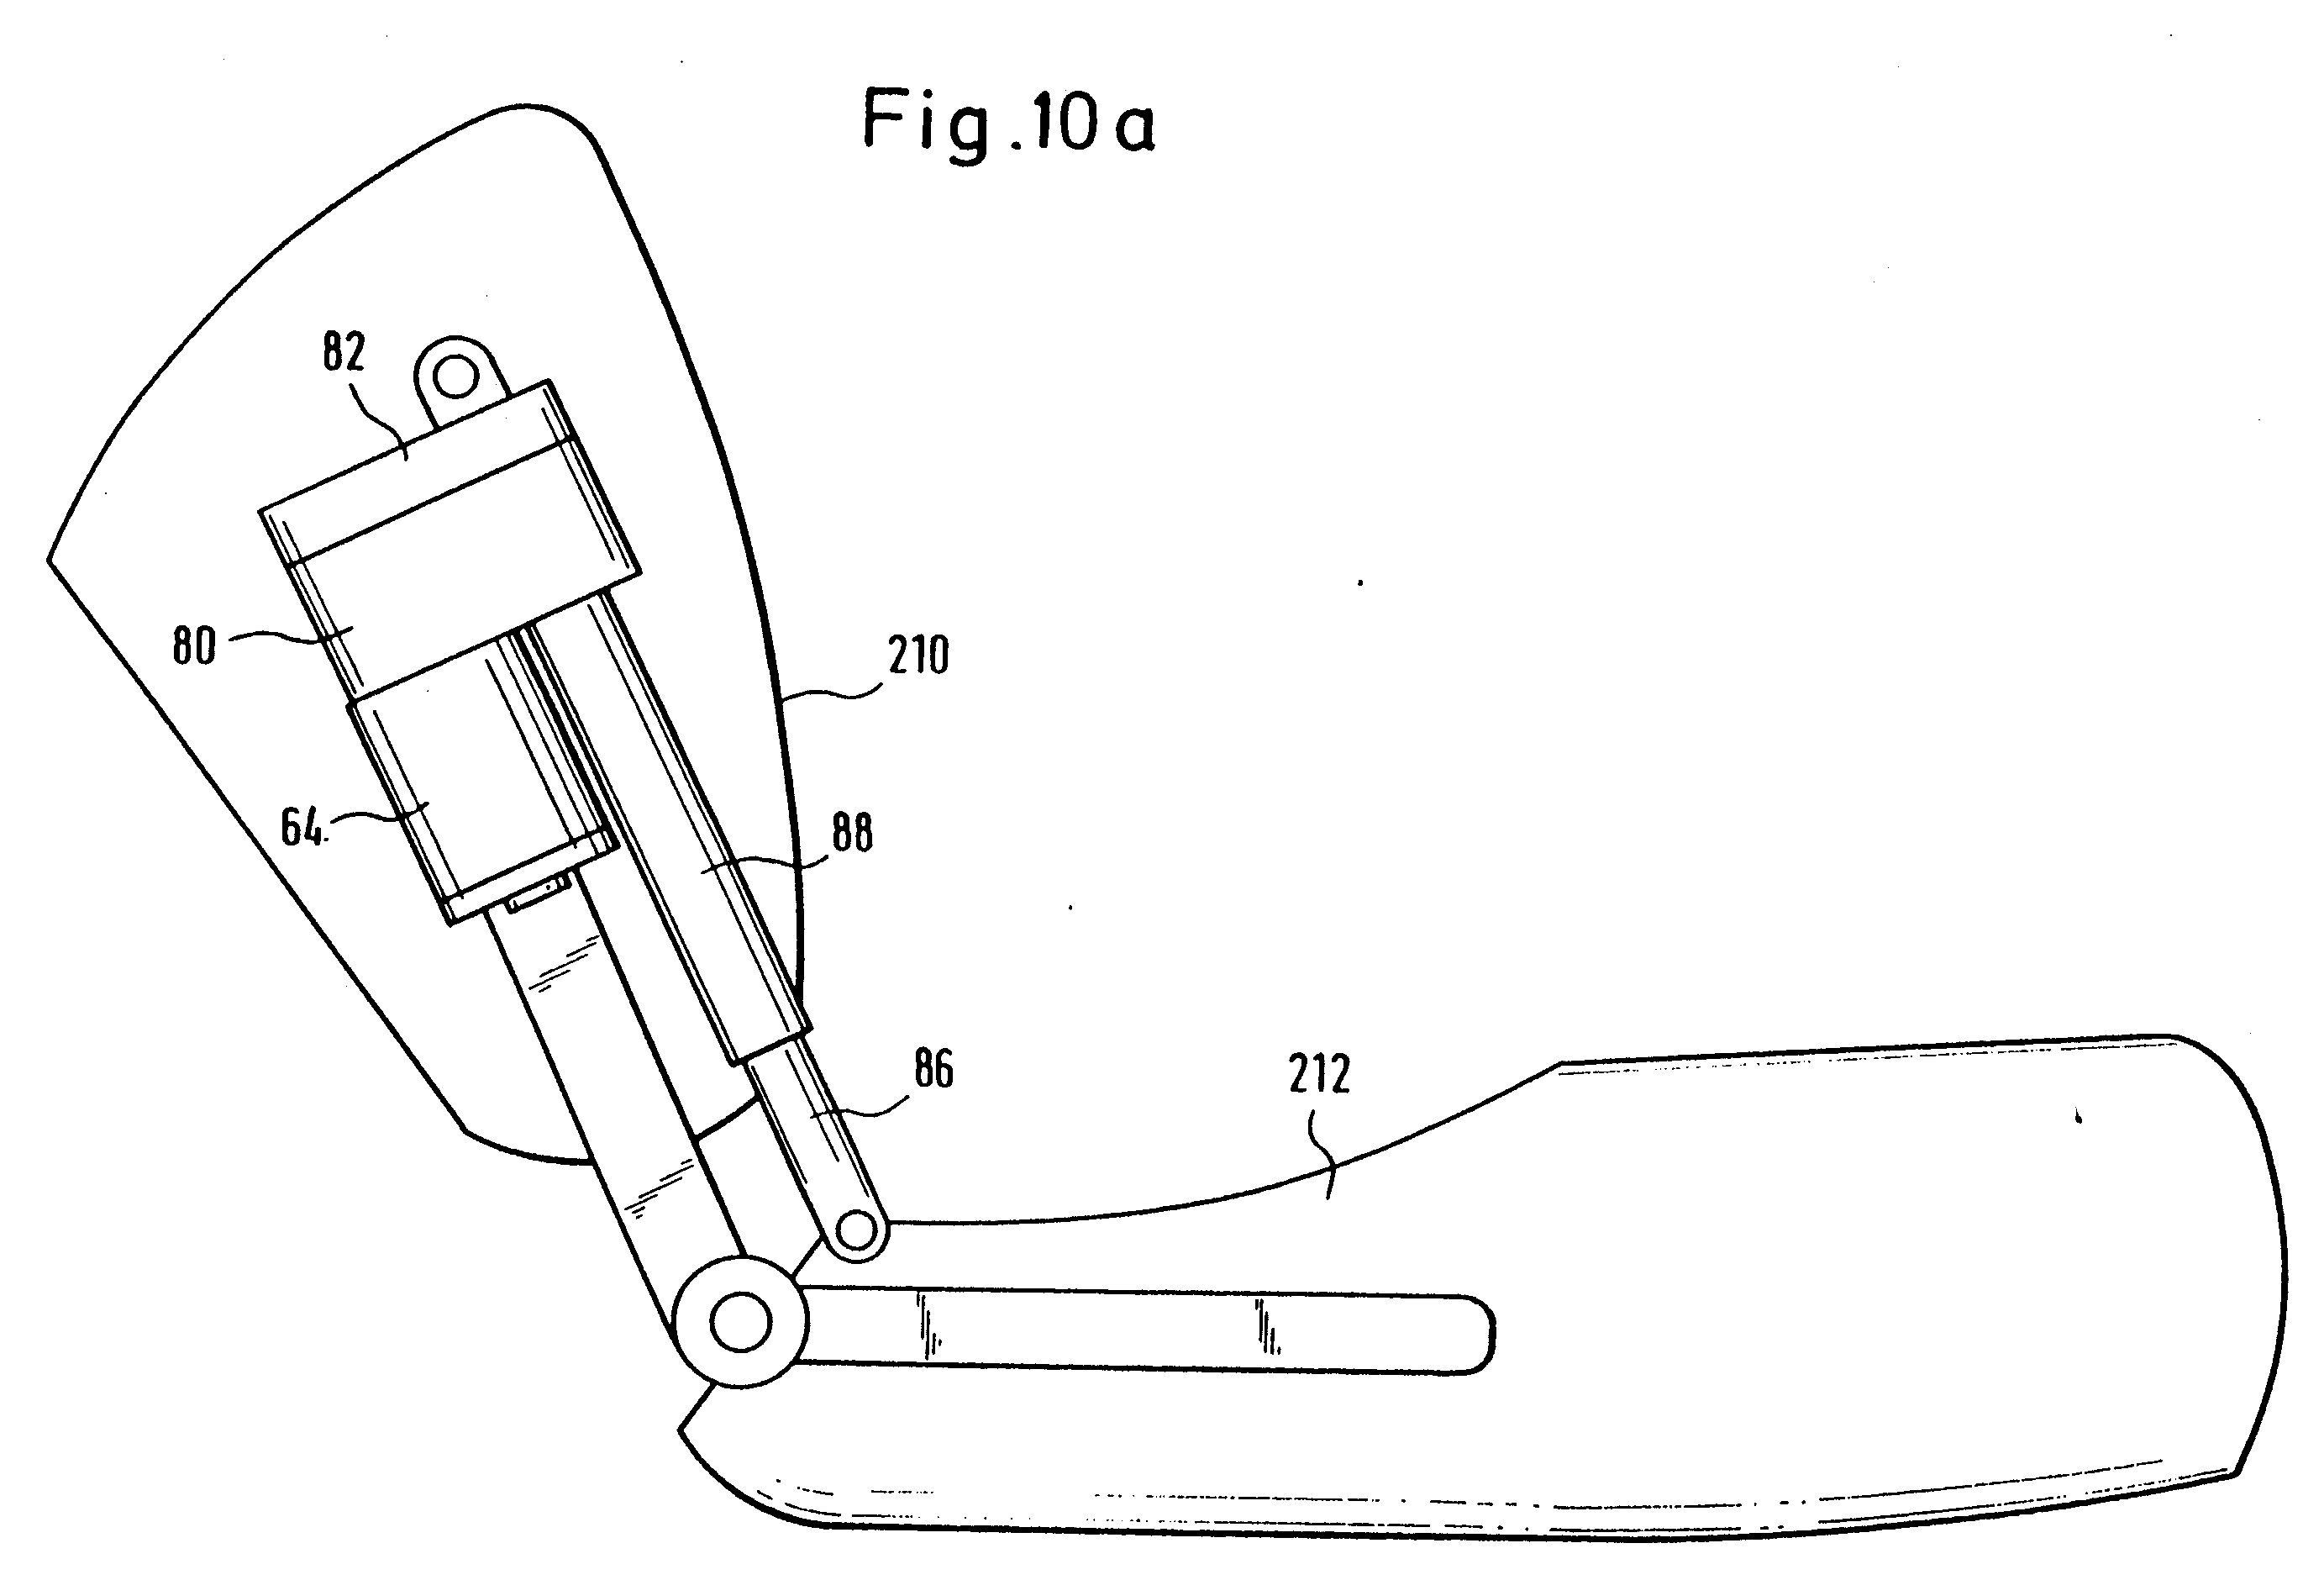
\includegraphics[width=0.54\linewidth]{US5252102_1.png}
  \caption{US5252102A apparatus with integrated electronic ROM sensing.}
  \label{fig:US5252102A}
\end{figure}

\subsection{Mechanism kinematics}
\begin{figure}[H]
  \centering
  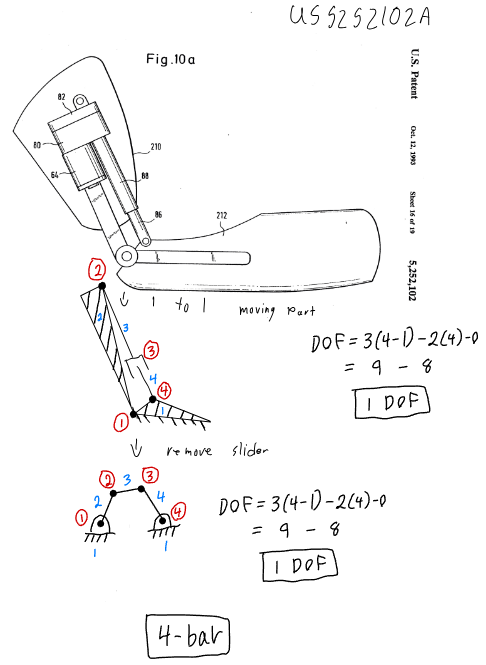
\includegraphics[width=0.54\linewidth]{../Kinematic Mechanism Images/5252102.png}
  \caption{Kinematics diagram for US5252102A electronic range of motion apparatus.}
  \label{fig:US5252102A_kinematics}
\end{figure}

\subsection{Degrees of Freedom}
\[
\begin{aligned}
DOF &= 3(n-1) - 2f_1 - f_2 \\
DOF &= 3(4-1) - 2(4) - 0 \\
DOF &= 1
\end{aligned}
\]

The mechanism has 1 degree of freedom and is a 4 bar linkage.

\subsection{Observations}
This patent integrates electronic sensing and feedback into a traditional CPM system, marking a transition toward data-driven rehabilitation. By recording range of motion and detecting resistance, the device enables clinicians to monitor patient progress quantitatively and ensure motion remains within safe limits. Mechanically, it retains a conventional linkage structure but augments it with position and torque sensors that provide valuable diagnostic data.

\subsection{Opportunities for Improvement}
Expanding this concept with wireless data transfer and cloud-based monitoring would modernize its functionality, allowing clinicians to review therapy sessions remotely. Pairing the sensing system with adaptive control could enhance safety and personalization. The particular advancements here preserve the patent's original focus on measurement and feedback while greatly improving accessibility and interactivity.

\section{US4492222A: Knee Exercise Machine}
\subsection{Description}
Knee exerciser that cyclically flexes the knee via a screw-driven leg support hinged to a thigh support and fixed to a motor assembly that pivots on a frame. Screw rotation within a tube advances/retracts the leg support; speed and flexion limit points are controllable.
\subsection{Images}
\begin{figure}[H]
  \centering
  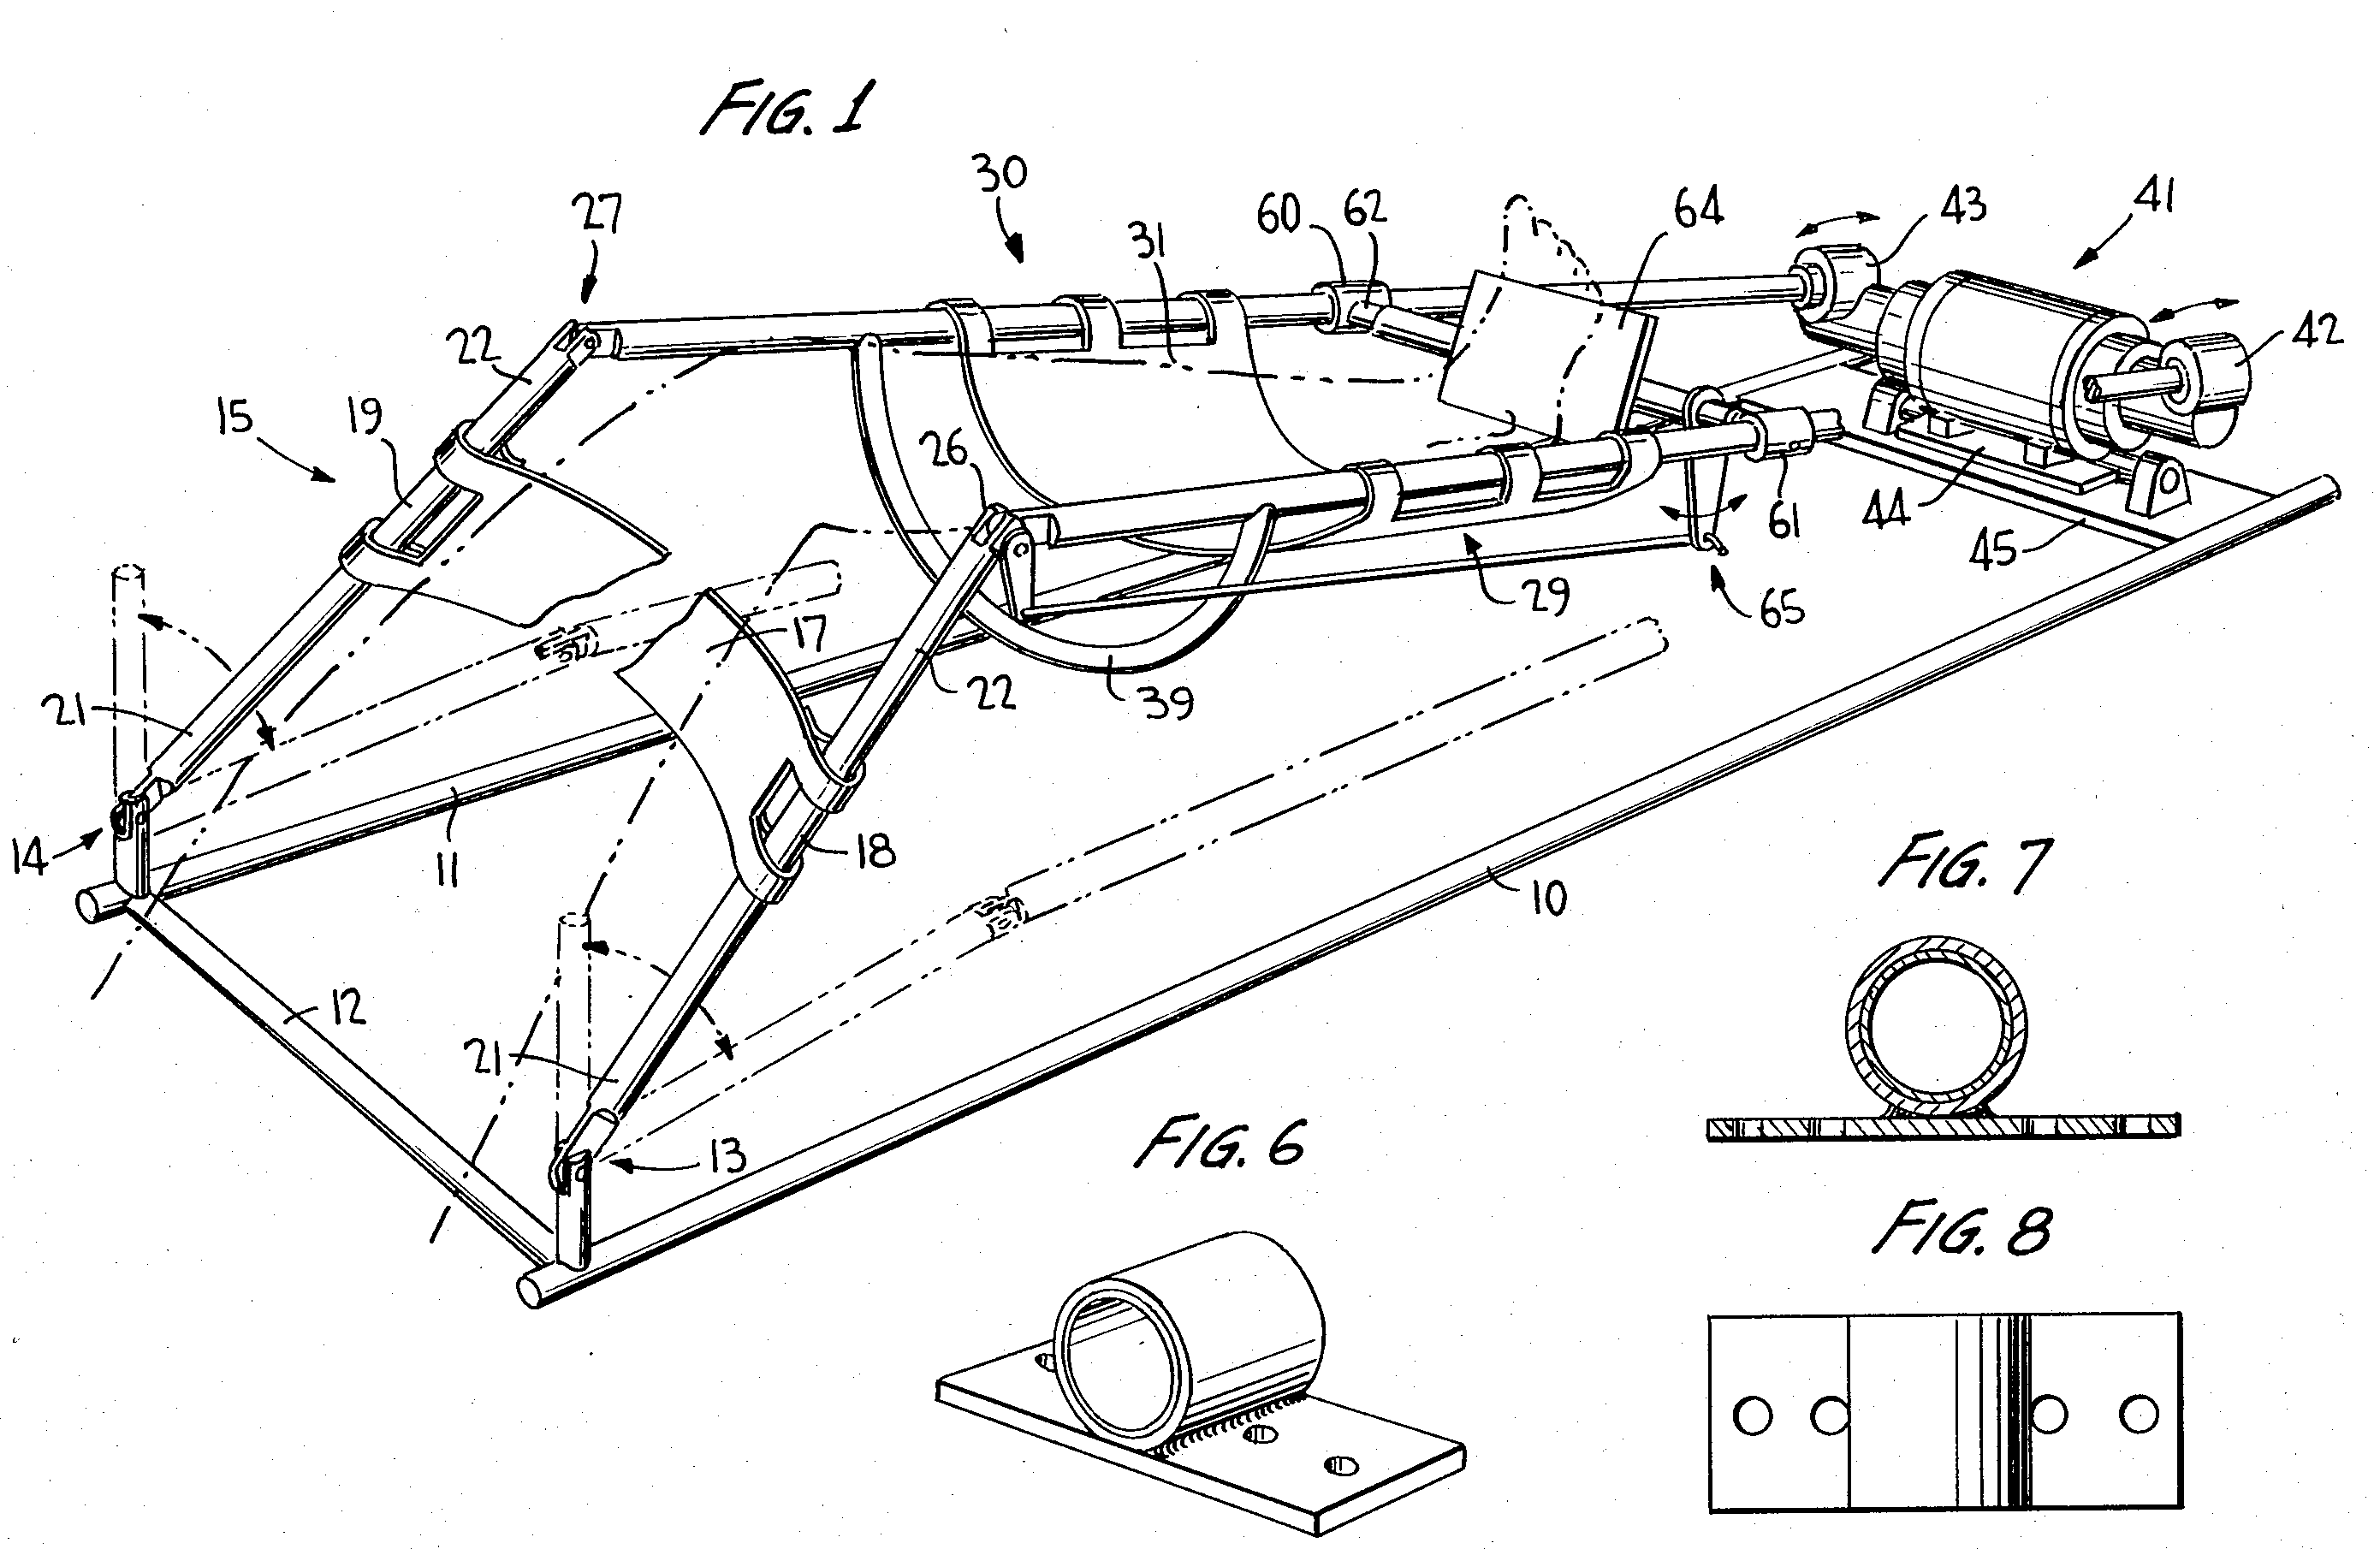
\includegraphics[width=0.54\linewidth]{4492222A_1.png}
  \caption{US4492222A knee exercise machine with adjustable axis alignment.}
  \label{fig:US4492222A}
\end{figure}

\subsection{Mechanism kinematics}
\begin{figure}[H]
  \centering
  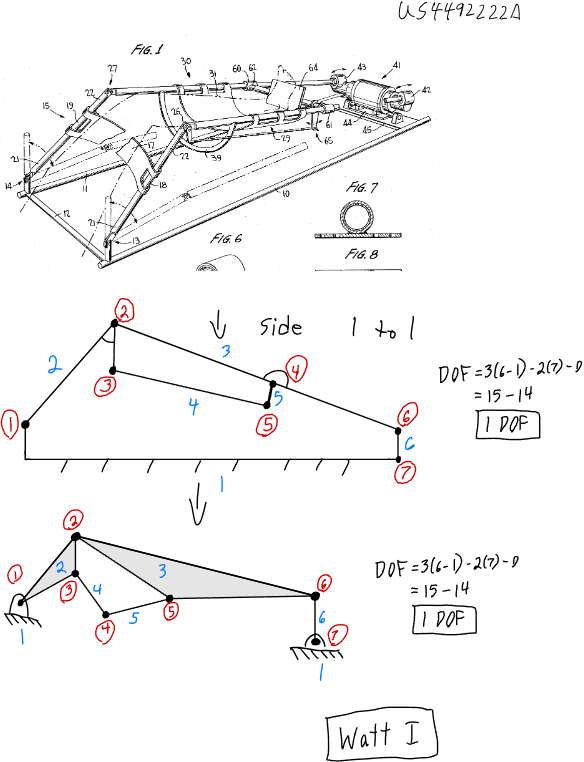
\includegraphics[width=0.54\linewidth]{../Kinematic Mechanism Images/4492222.png}
  \caption{Kinematics diagram for US4492222A knee exercise machine.}
  \label{fig:US4492222A_kinematics}
\end{figure}

\subsection{Degrees of Freedom}
\[
\begin{aligned}
DOF &= 3(n-1) - 2f_1 - f_2 \\
DOF &= 3(6-1) - 2(7) - 0 \\
DOF &= 1
\end{aligned}
\]

The mechanism has 1 degree of freedom and is a Watt I mechanism.

\subsection{Observations}
This patent shows a mechanical knee exercise machine with a focus on axis alignment between femoral and tibial supports. The system is adjustable, allowing clinicians to fine tune the mechanical pivot to match individual anatomy. This capability reduces off axis loading and enhances the accuracy of joint motion replication. The bulk and manual adjustment requirements may hinder usability in nonclinical environments.

\subsection{Opportunities for Improvement}
Streamlining the adjustment process through indexed or self-aligning pivots could make setup faster and more intuitive, minimizing the potential for misalignment. Introducing foldable or modular components would further expand its usability beyond clinic settings. These changes would modernize the design while preserving its core advantage of accurate joint axis alignment.

\section{US10272291B2: Knee Flexion and Extension Therapy Device and Method of Use}
\subsection{Description}
Portable exercise board with a sliding foot board/seat slide and removable knee/ankle platform for active or passive knee extension stretching and short-arc quadriceps work. Fixed and moving indices mark progress, and sensors plus a controller or smart device provide visual/auditory feedback for controlled flexion/extension.
\subsection{Images}
\begin{figure}[H]
  \centering
  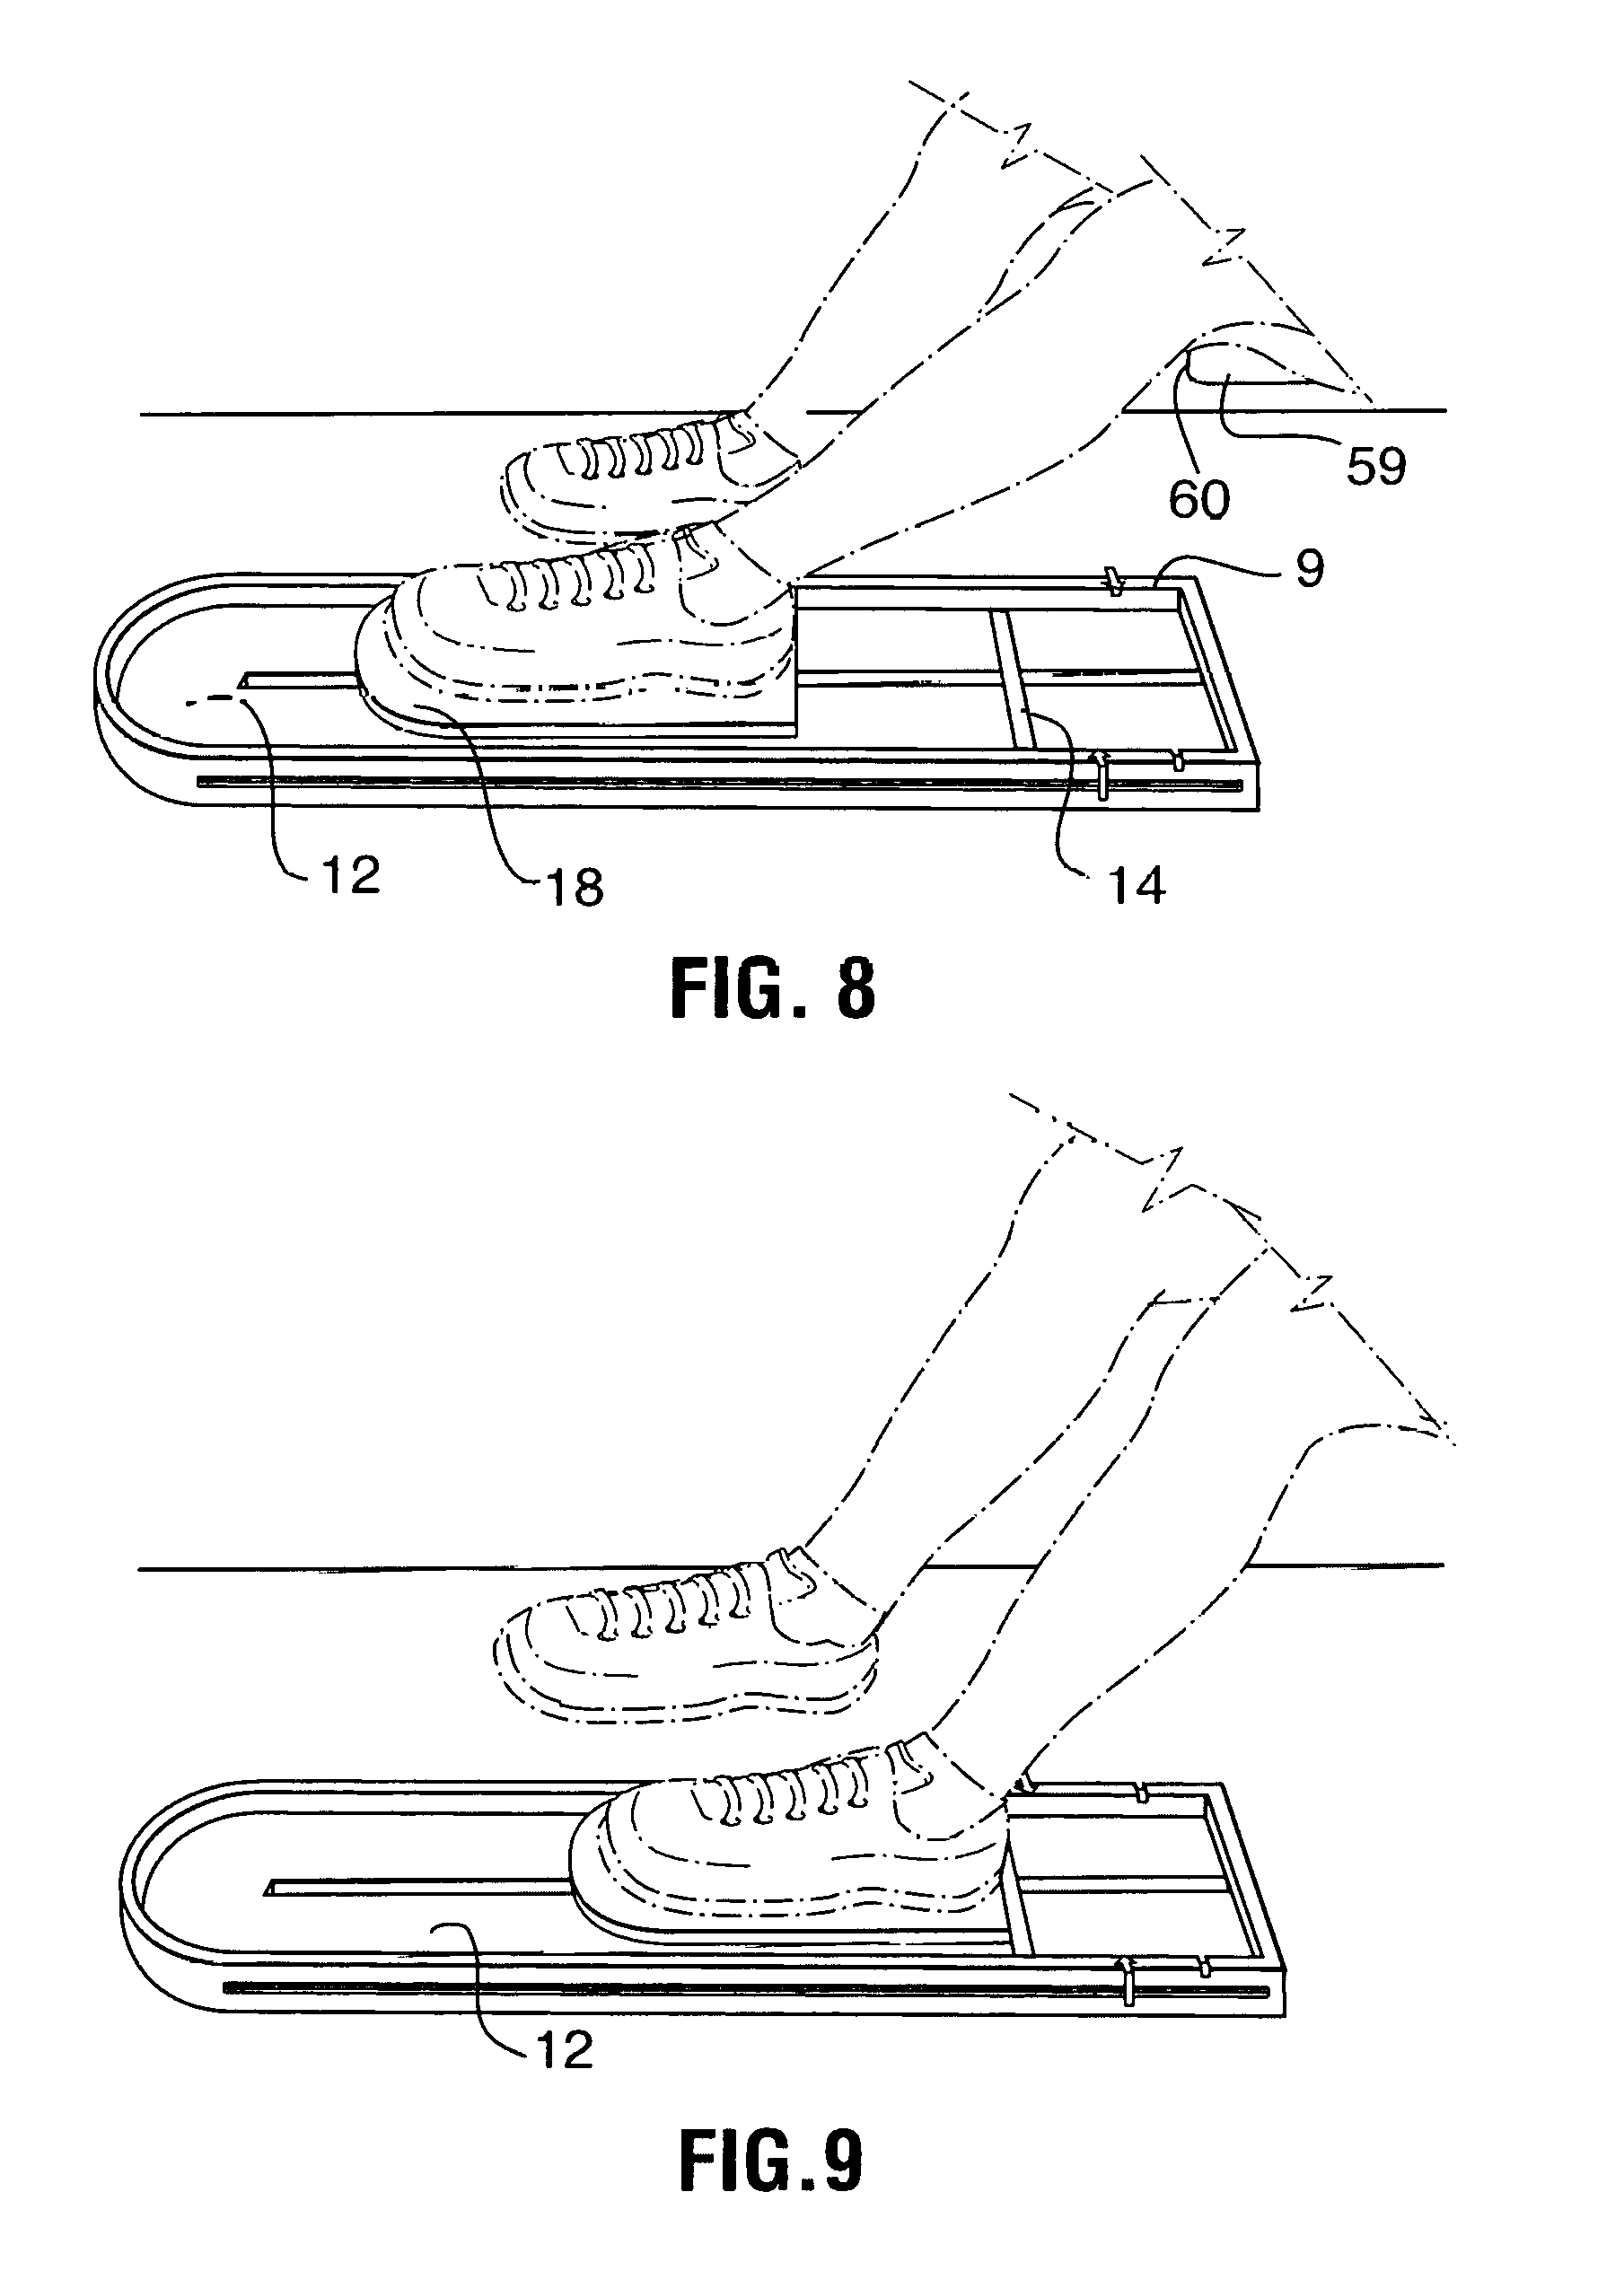
\includegraphics[width=0.54\linewidth]{10272291B2_1.png}
  \caption{US10272291B2 modern therapy platform for knee flexion/extension.}
  \label{fig:US10272291B2}
\end{figure}

\subsection{Mechanism kinematics}
\begin{figure}[H]
  \centering
  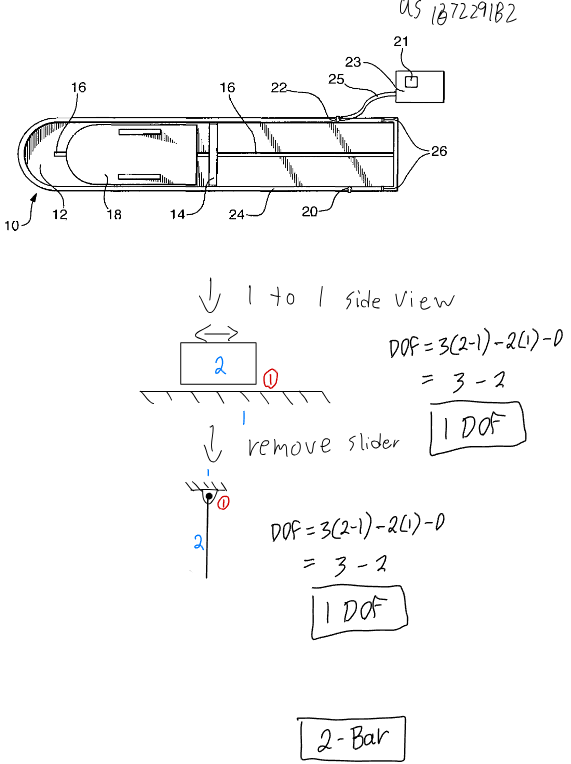
\includegraphics[width=0.54\linewidth]{../Kinematic Mechanism Images/10272291.png}
  \caption{Kinematics diagram for US10272291B2 knee flexion and extension therapy device.}
  \label{fig:US10272291B2_kinematics}
\end{figure}

\subsection{Degrees of Freedom}
\[
\begin{aligned}
DOF &= 3(n-1) - 2f_1 - f_2 \\
DOF &= 3(2-1) - 2(1) - 0 \\
DOF &= 1
\end{aligned}
\]

The mechanism is a simple slider mechanism with 1 degree of freedom.

\subsection{Observations}
This patent reflects a significant evolution in CPM technology, integrating digital sensors, modular components, and portable design features to accommodate both clinical and at home use. The mechanism combines traditional linkage motion with embedded encoders or inertial sensors for real time tracking of angular position and speed. The use of lightweight materials and adjustable limb supports demonstrates attention to ergonomics and patient comfort. The system's modularity also suggests compatibility with mobile data systems for progress monitoring. The inclusion of multiple electronic subsystems introduces potential reliability and power management challenges that earlier mechanical designs avoided.

\subsection{Opportunities for Improvement}
Enhancements could focus on improving usability and energy efficiency through better battery management and intuitive software interfaces. Simplified clinician presets and patient guided setup routines could reduce user error while maintaining precise control. Integrating cloud connectivity for data storage and remote supervision would further align the device with current trends in tele-rehabilitation. These refinements would enhance the balance between technological sophistication and practical reliability, ensuring the device remains accessible while offering advanced monitoring and control.

\section{US4603687A: Continuous Passive Motion Orthopedic Device}
\subsection{Description}
Orthopedic CPM device employing counterbalanced support arms and a motorized actuator to deliver steady cyclic motion while minimizing off-axis loads; includes alignment aids and adjustable supports for consistent articulation.
\subsection{Images}
\begin{figure}[H]
  \centering
  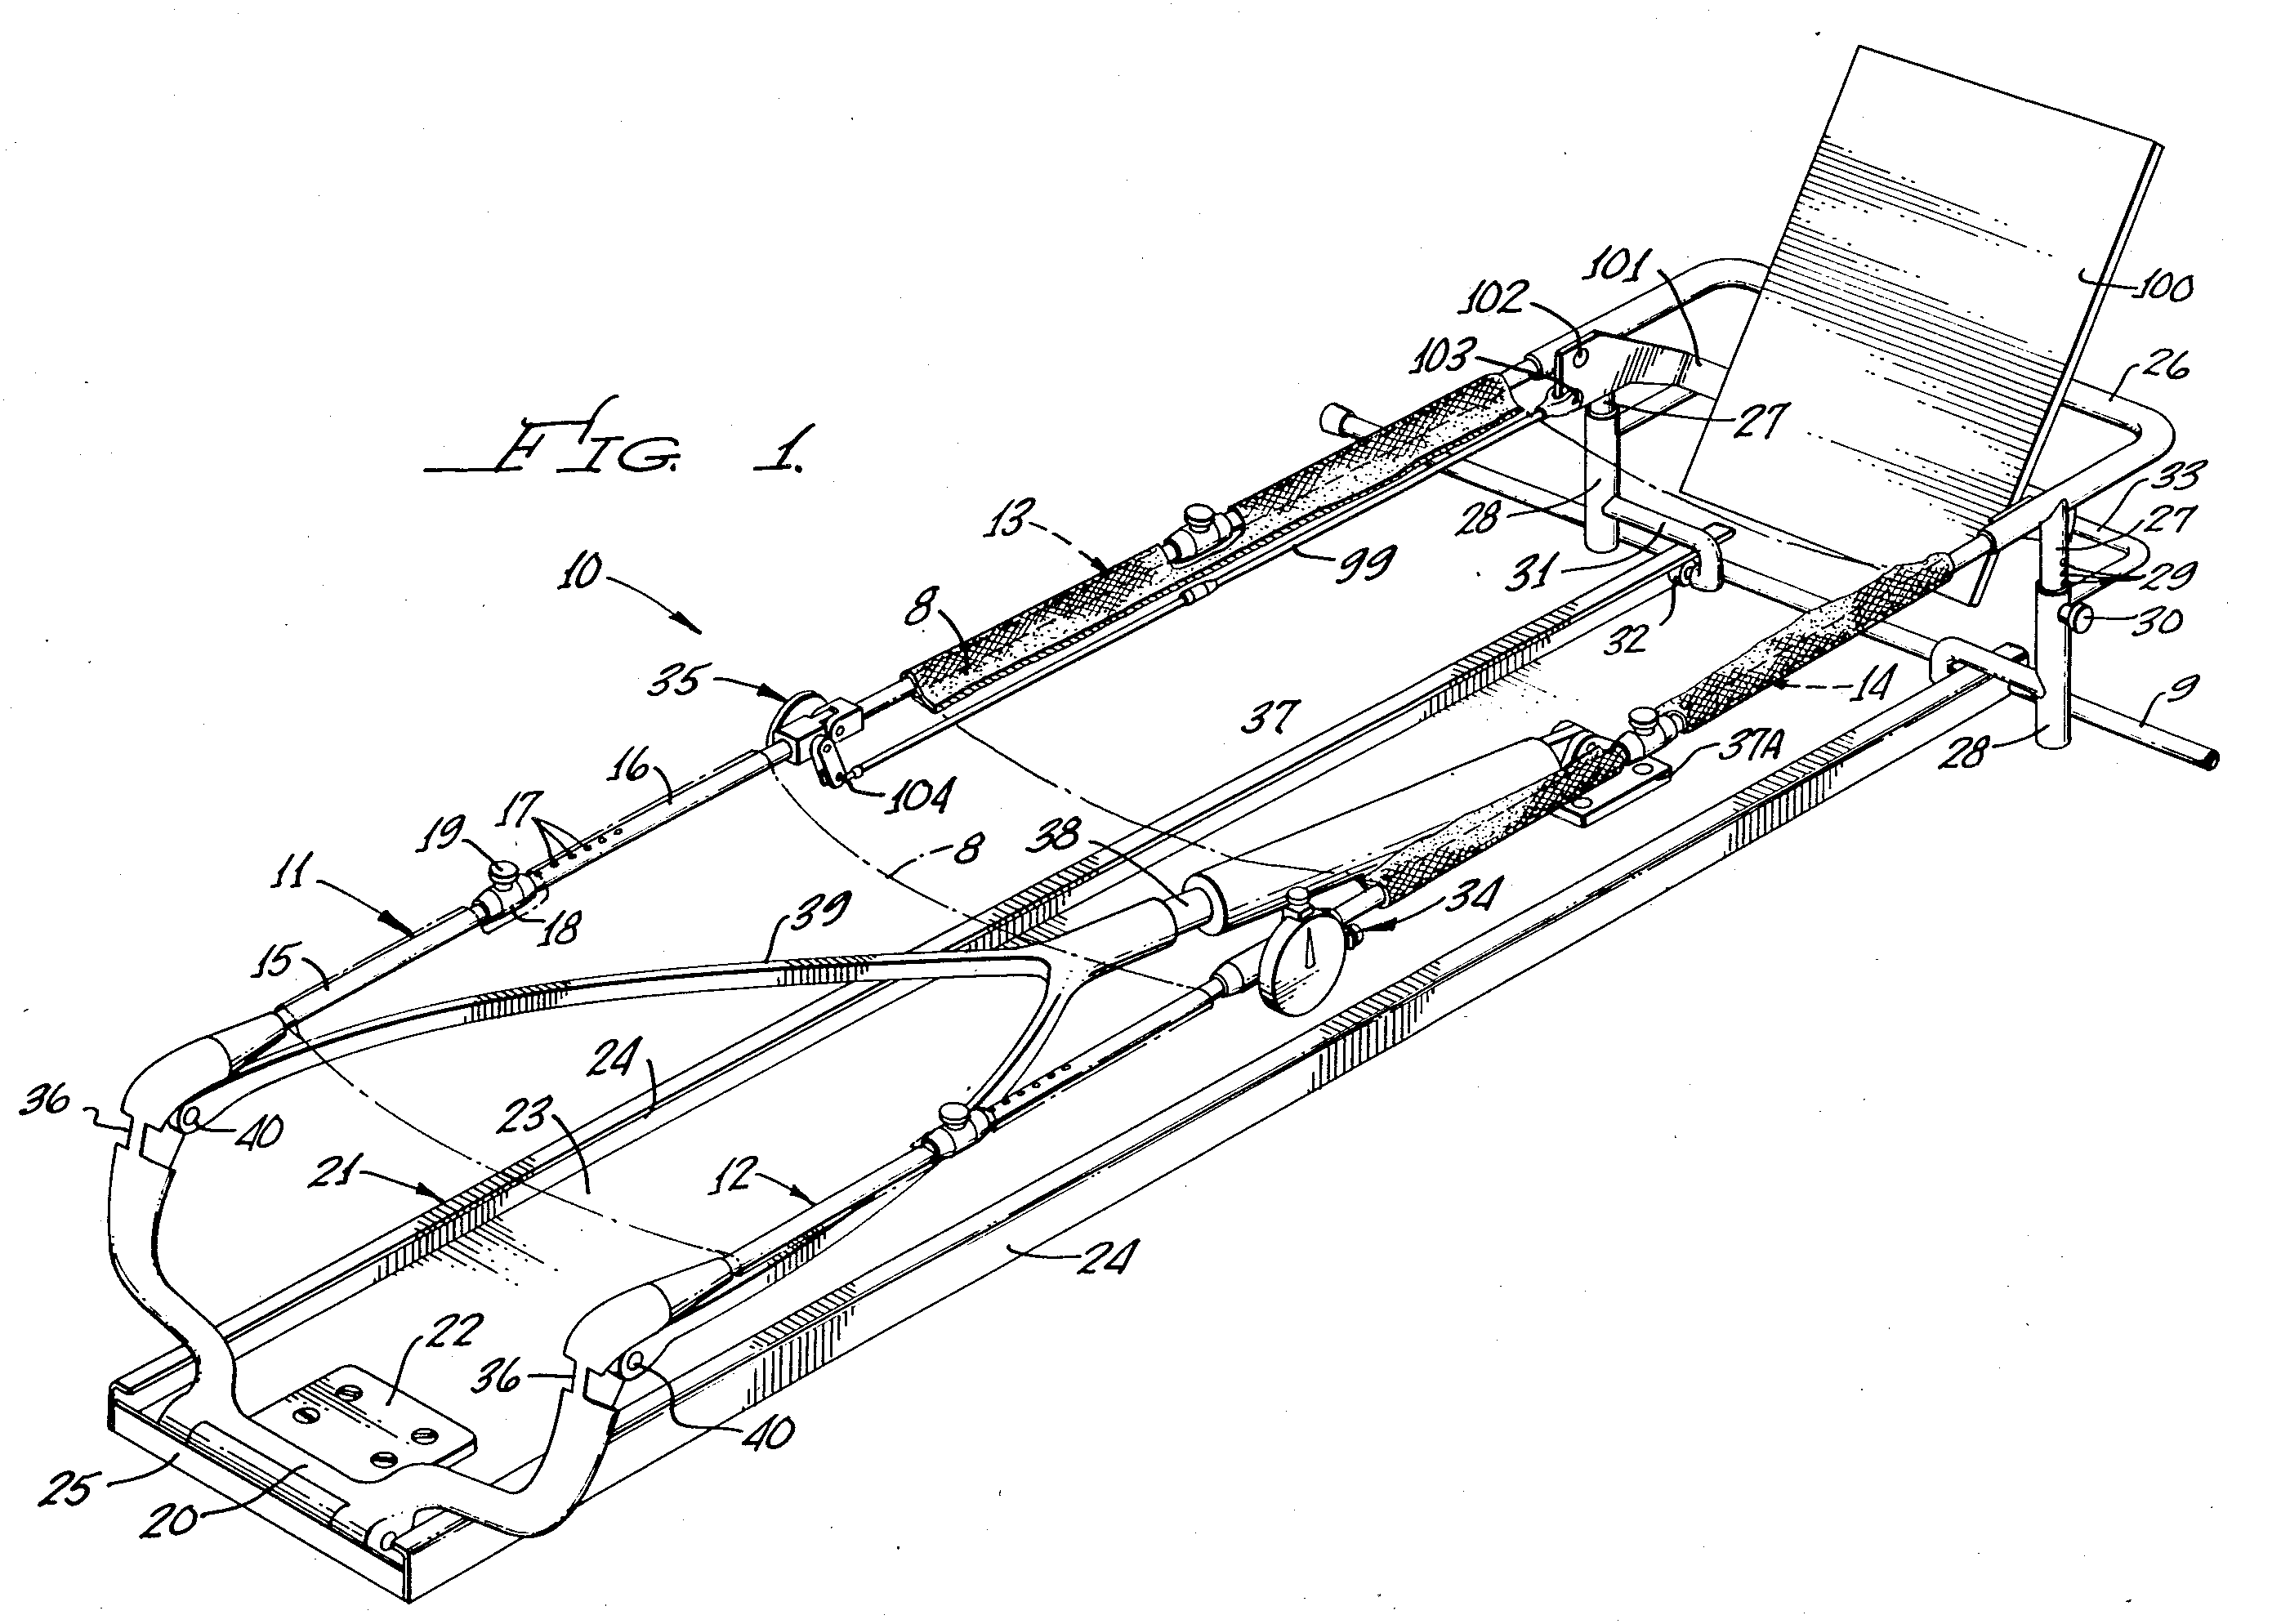
\includegraphics[width=0.54\linewidth]{US4603687_1.png}
  \caption{US4603687A CPM with counterbalanced arms and alignment aids.}
  \label{fig:US4603687A}
\end{figure}

\subsection{Mechanism kinematics}
\begin{figure}[H]
  \centering
  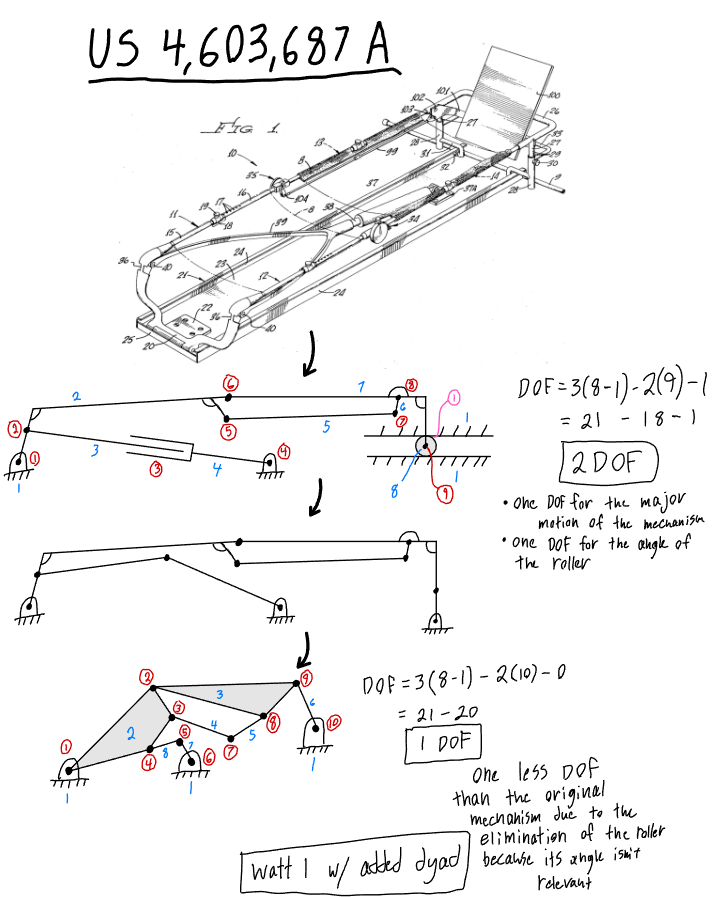
\includegraphics[width=0.54\linewidth]{../Kinematic Mechanism Images/4603687.png}
  \caption{Kinematics diagram for US4603687A continuous passive motion orthopedic device.}
  \label{fig:US4603687A_kinematics}
\end{figure}

\subsection{Degrees of Freedom}
\[
\begin{aligned}
DOF &= 3(n-1) - 2f_1 - f_2 \\
DOF &= 3(8-1) - 2(10) - 0 \\
DOF &= 1
\end{aligned}
\]

The mechanism, neglecting the roller rotation, has 1 degree of freedom and is a Watt I mechanism with an added dyad.

\subsection{Observations}
This design incorporates counterbalanced support arms to reduce the torque demands on the drive motor and minimize the physical strain on the patient. The use of balanced linkages allows smoother operation and consistent motion profiles across a range of limb weights, representing a thoughtful mechanical optimization. By improving load distribution, the design also enhances safety and reduces actuator wear. However, its relatively large frame and reliance on rigid structural components make the system heavy and less adaptable for different rehabilitation environments.

\subsection{Opportunities for Improvement}
Replacing bulky counterweights with compact spring based or pneumatic balancing systems could significantly reduce size and weight while maintaining equilibrium. Introducing adjustable counterbalance calibration would enable use across a wider range of patients without manual recalibration. Furthermore, using advanced lightweight alloys or composite arms could further reduce inertia, improving responsiveness and portability. These updates would retain the patent's core mechanical advantage while modernizing its form factor and usability.

\section{US5239987A: Anatomically Correct Continuous Passive Motion Device for a Limb}
\subsection{Description}
Axis-following CPM that accommodates the knee’s migrating instantaneous center of rotation by guiding the limb along a more anatomic “J-curve,” reducing misalignment-induced shear during passive motion.
\subsection{Images}
\begin{figure}[H]
  \centering
  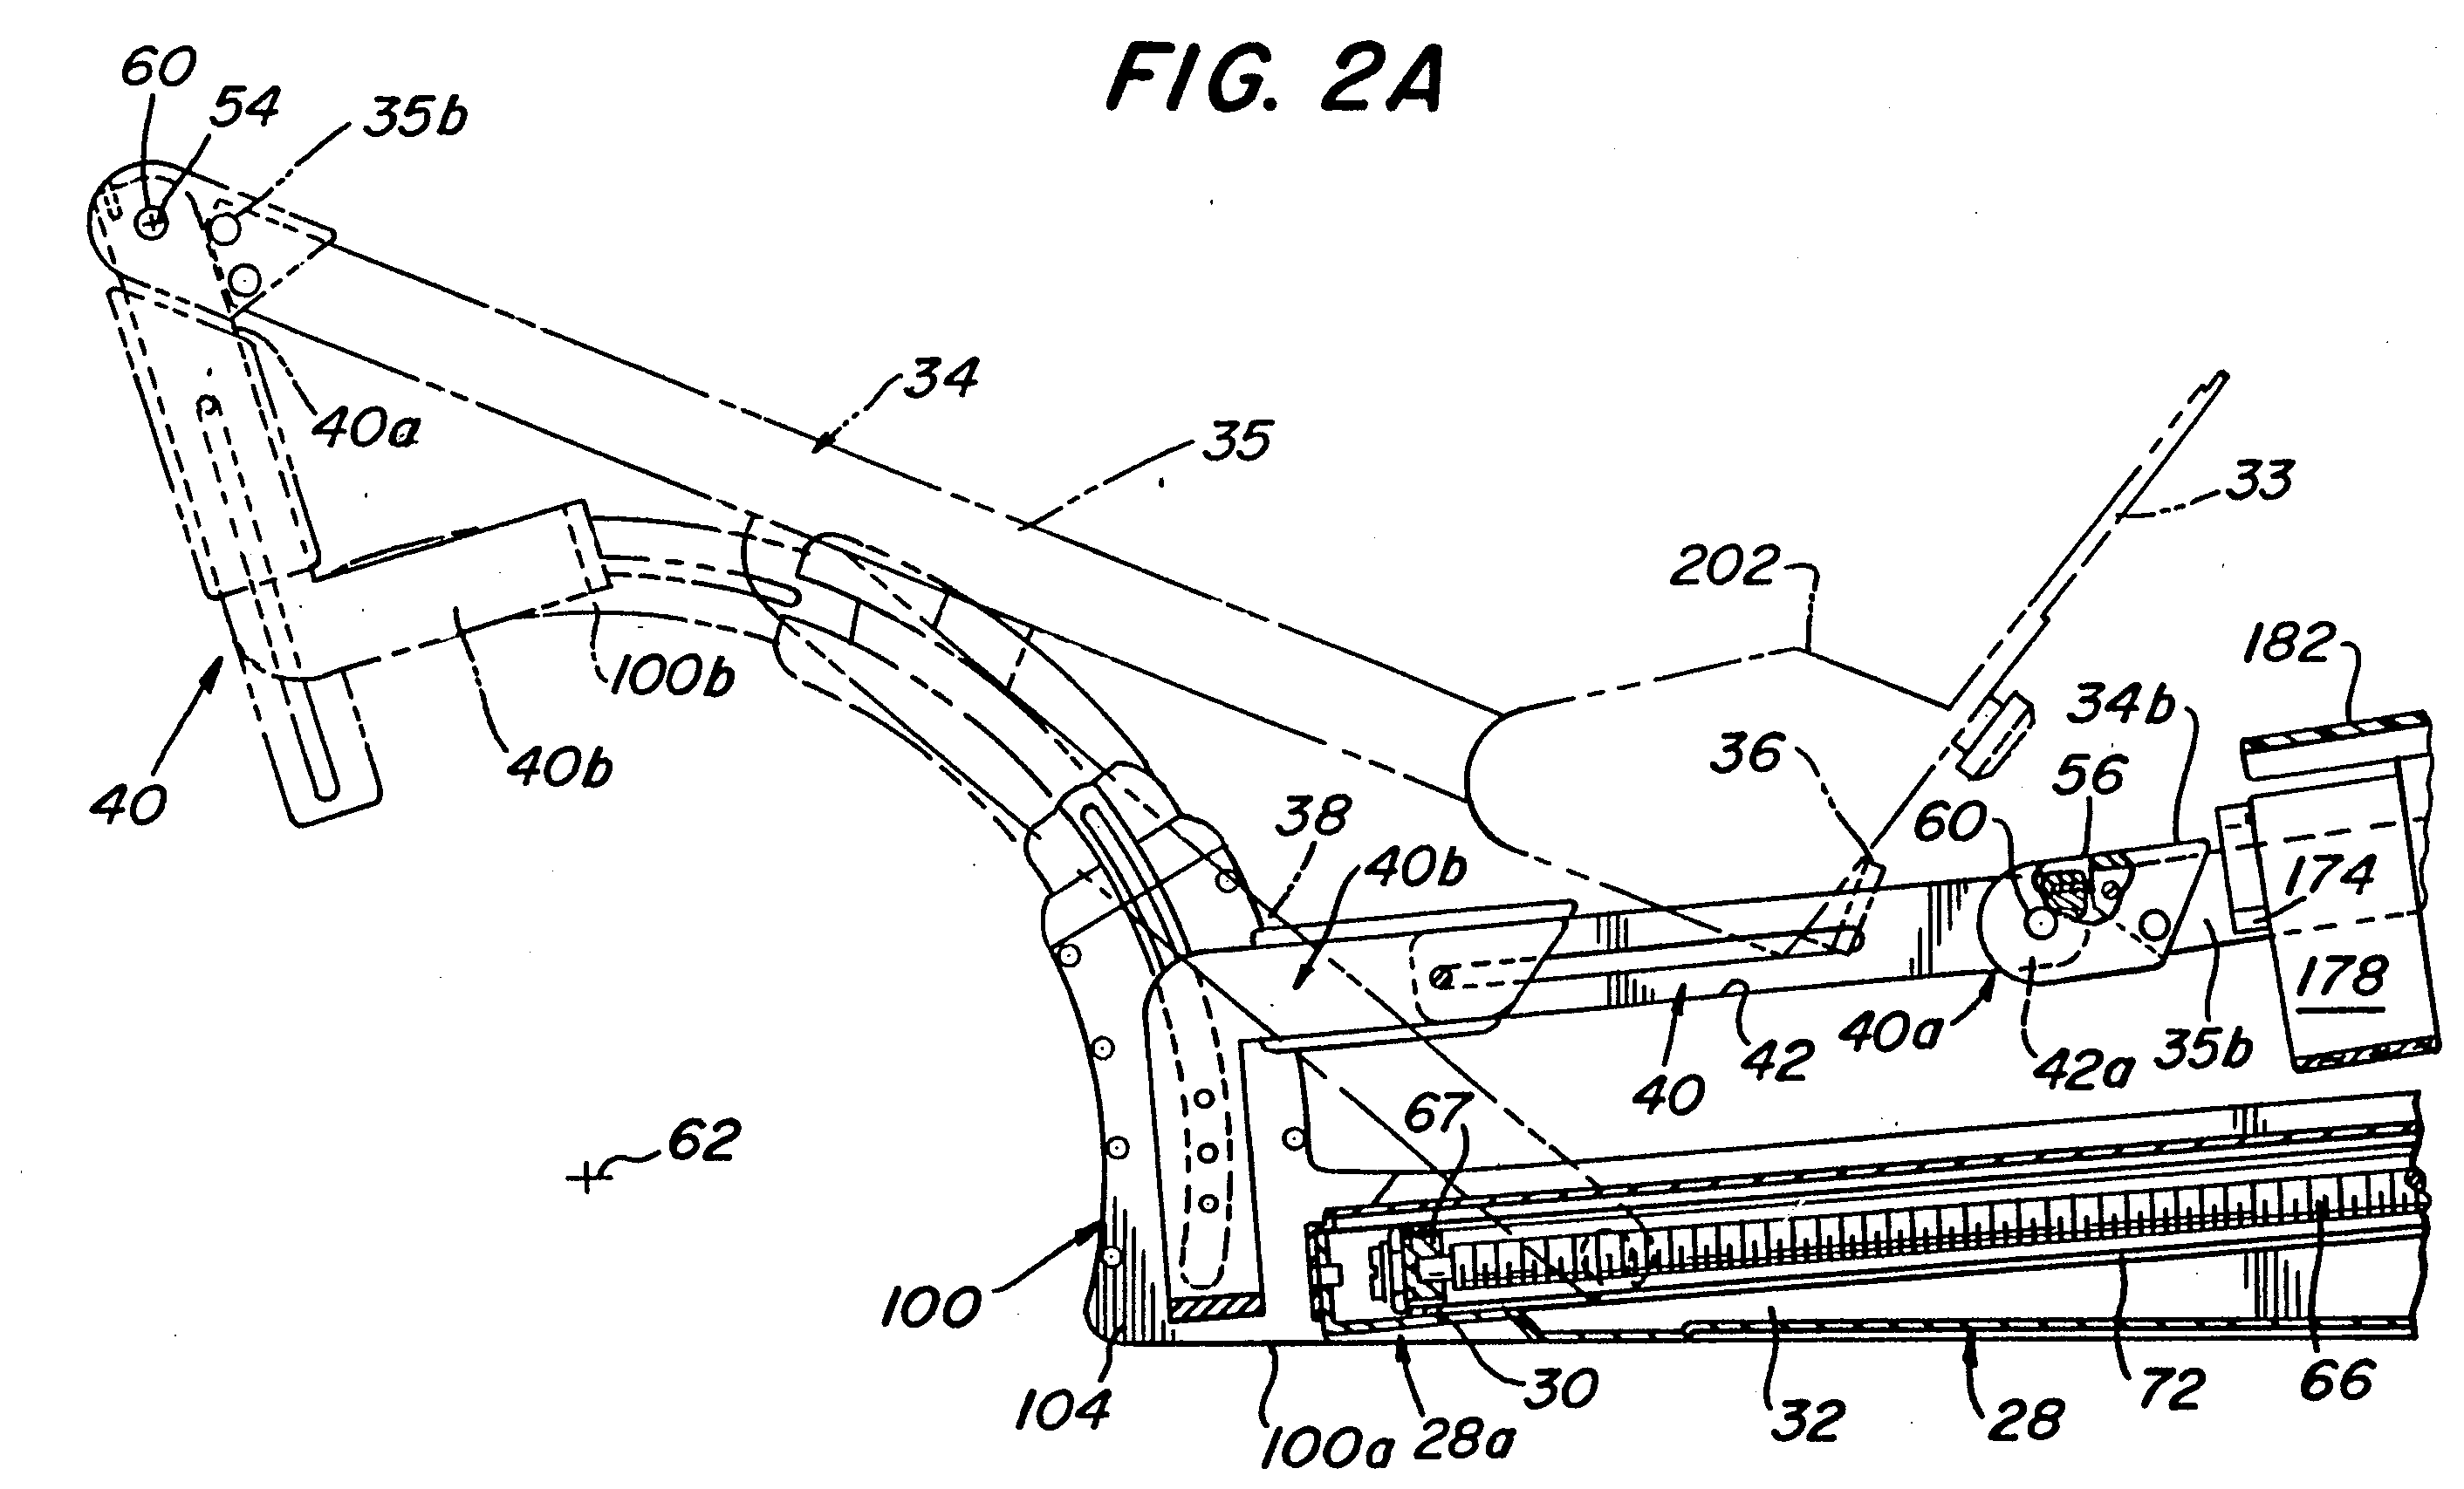
\includegraphics[width=0.54\linewidth]{US5239987-drawings-page-3.png}
  \caption{US5239987A device adapting to the knee’s shifting rotation center.}
  \label{fig:US5239987A}
\end{figure}

\subsection{Mechanism kinematics}
\begin{figure}[H]
  \centering
  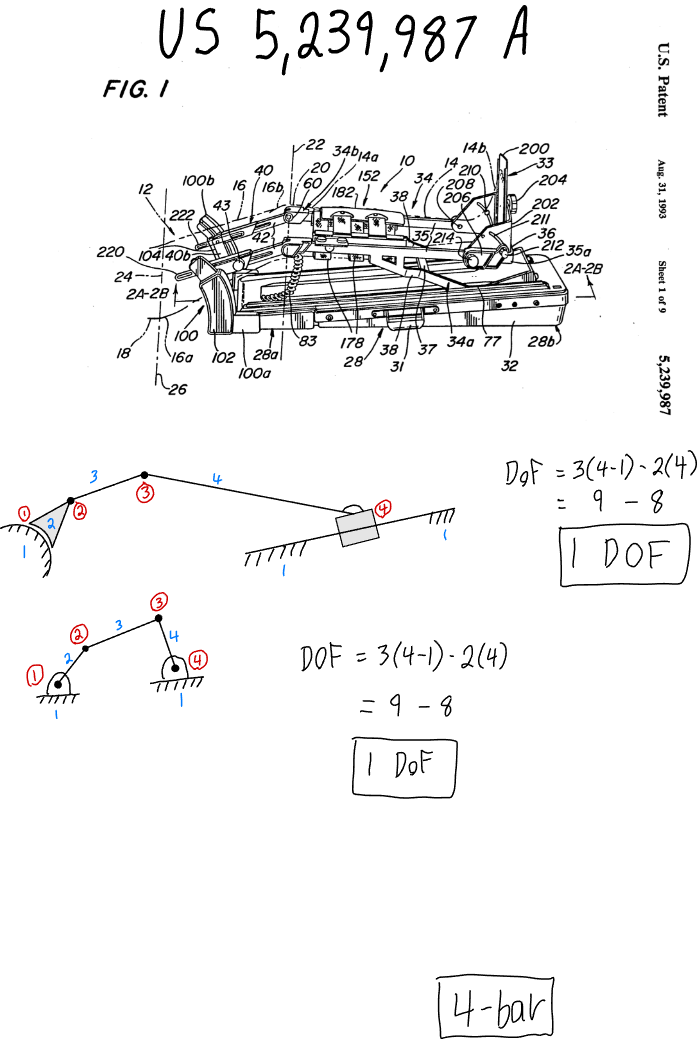
\includegraphics[width=0.54\linewidth]{../Kinematic Mechanism Images/5239987.png}
  \caption{Kinematics diagram for US5239987A anatomically correct continuous passive motion device.}
  \label{fig:US5239987A_kinematics}
\end{figure}

\subsection{Degrees of Freedom}
\[
\begin{aligned}
DOF &= 3(n-1) - 2f_1 - f_2 \\
DOF &= 3(4-1) - 2(4) - 0 \\
DOF &= 1
\end{aligned}
\]

The mechanism has 1 degree of freedom and is a 4 bar linkage.

\subsection{Observations}
This patent focuses on replicating the knee's natural instantaneous center of rotation by employing an axis-following or ``J-curve'' linkage path. The design represents a sophisticated application of kinematic synthesis to orthopedic rehabilitation, allowing more anatomically accurate motion that reduces shear forces and enhances comfort. Such precision comes at the cost of mechanical complexity, requiring tight tolerances and careful calibration. While the anatomical fidelity is a major advancement, manufacturing difficulty and setup sensitivity likely limited its widespread adoption.

\subsection{Opportunities for Improvement}
Future designs could pursue simplified link arrangements. An optimized four-bar or compliant mechanism that preserves the J-curve motion with fewer components is one line of thinking. Adjustable link geometries could allow clinicians to tune motion profiles to individual patients without custom fabrication. Integrating sensors to verify axis alignment during setup could further improve reliability. These refinements would maintain the device's biomechanical accuracy while improving manufacturability and ease of use, making anatomically correct CPM more practical for routine clinical application.

\section{US4546763A: Continuous Passive Motion Method and Apparatus}
\subsection{Description}
Claims both the CPM apparatus and protocol features including programmable cycle timing, dwell at end range, and progressive ROM to standardize therapy dosing with reliable mechanical delivery.
\subsection{Images}
\begin{figure}[H]
  \centering
  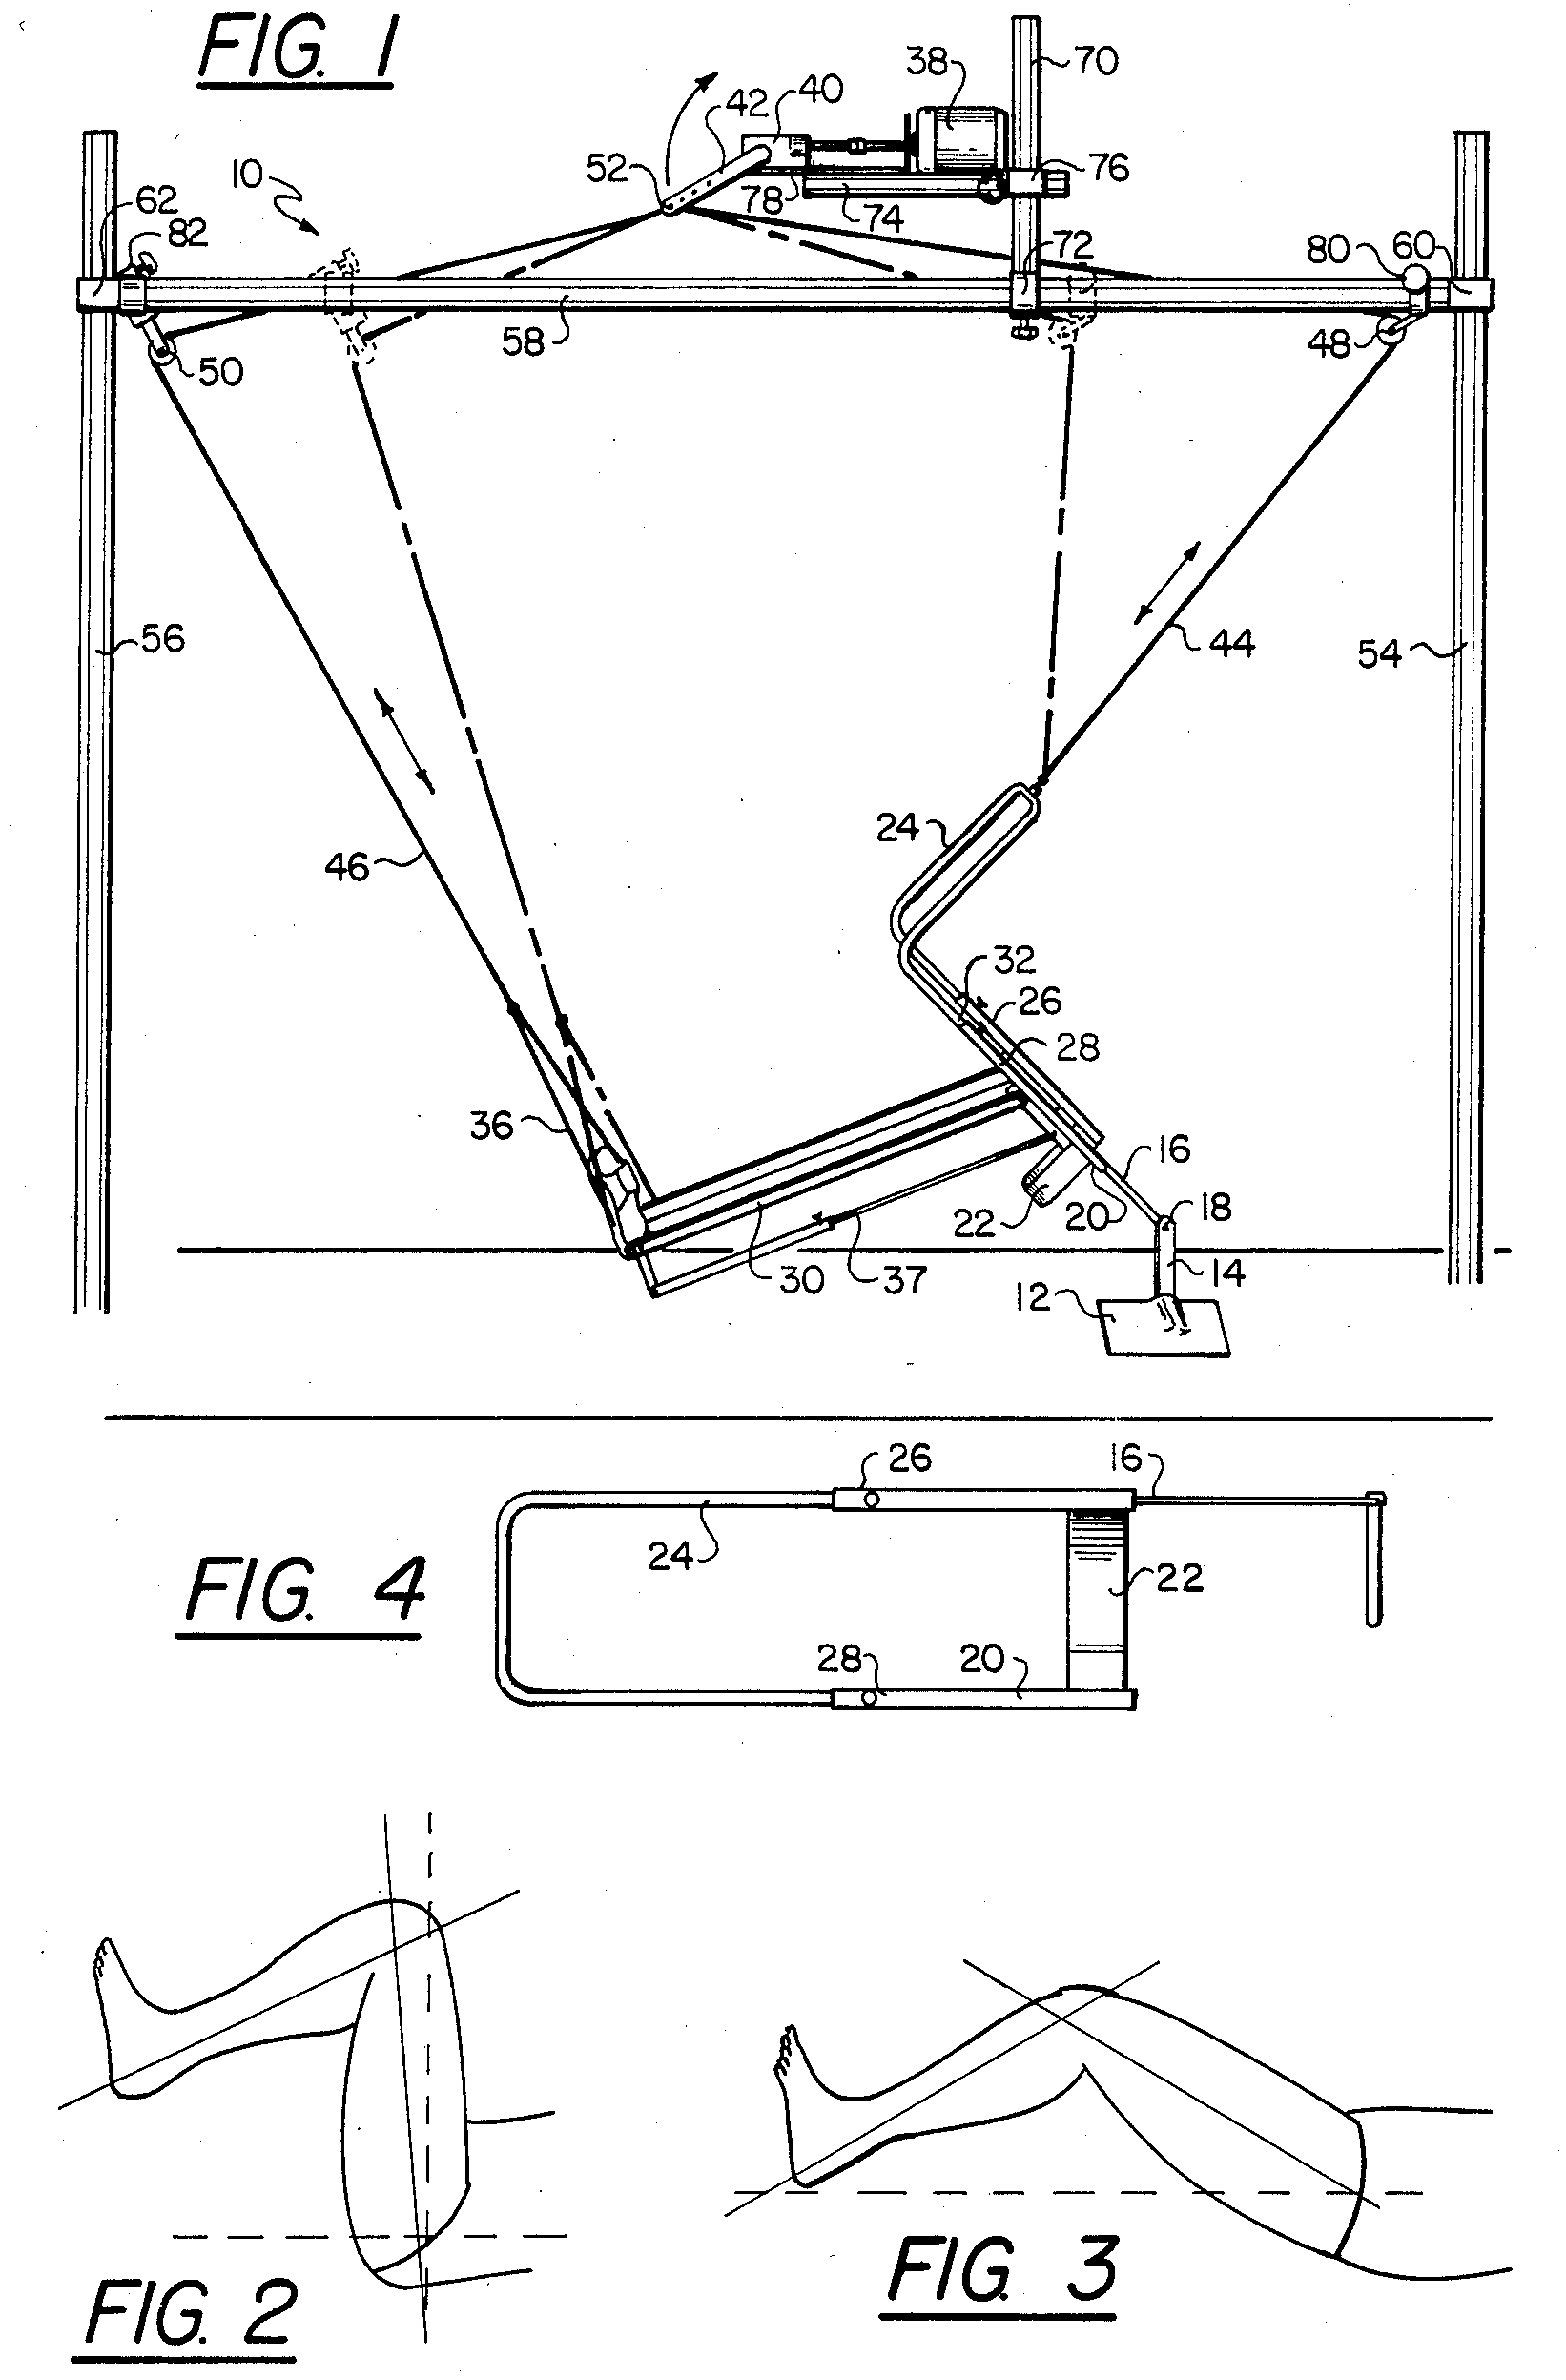
\includegraphics[width=0.54\linewidth]{US4546763-drawings-page-2.png}
  \caption{US4546763A apparatus and protocol emphasizing programmable CPM dosing.}
  \label{fig:US4546763A}
\end{figure}

\subsection{Mechanism kinematics}
\begin{figure}[H]
  \centering
  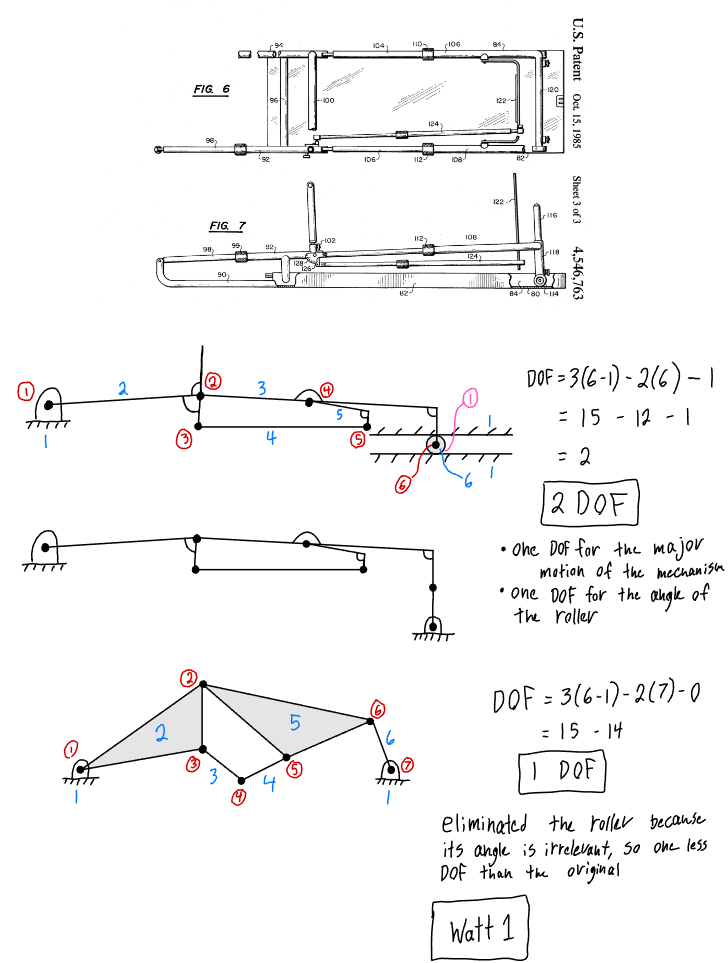
\includegraphics[width=0.54\linewidth]{../Kinematic Mechanism Images/4546763.png}
  \caption{Kinematics diagram for US4546763A continuous passive motion method and apparatus.}
  \label{fig:US4546763A_kinematics}
\end{figure}

\subsection{Degrees of Freedom}
\[
\begin{aligned}
DOF &= 3(n-1) - 2f_1 - f_2 \\
DOF &= 3(6-1) - 2(7) - 0 \\
DOF &= 1
\end{aligned}
\]

The mechanism has 1 degree of freedom and is a Watt I mechanism.

\subsection{Observations}
This patent combines a mechanical device with defined therapeutic protocols, emphasizing programmable timing, dwell intervals, and progressive range of motion. It marks a shift toward evidence-based rehabilitation through repeatable motion dosing. Mechanically, it employs a conventional motor driven linkage system, but the innovation lies in its programmable controller, which enables consistent execution of therapy regimens. This hybrid of engineering and clinical insight underscores the importance of standardized therapy but still depends heavily on manual input and static programming.

\subsection{Opportunities for Improvement}
Integrating adaptive control algorithms that respond to patient feedback such as pain inputs, motion resistance, or compliance would evolve the system into a truly intelligent therapy platform. Cloud based storage and analytics could allow clinicians to monitor outcomes and adjust protocols remotely. User friendly software interfaces with built in clinical presets would further simplify setup and improve adherence. By modernizing the control strategy while maintaining the patent's commitment to repeatable, evidence based motion, future designs could bridge the gap between mechanical precision and personalized therapy.

\section{US4637379A: Device for Imparting Continuous Passive Motion to Leg Joints}
\subsection{Description}
CPM device for leg joints that translates linear carriage motion into combined longitudinal and arcuate displacement of a foot rest; supports selective mobilization of hip/knee together or ankle alone by changing pivot constraints.
\subsection{Images}
\begin{figure}[H]
  \centering
  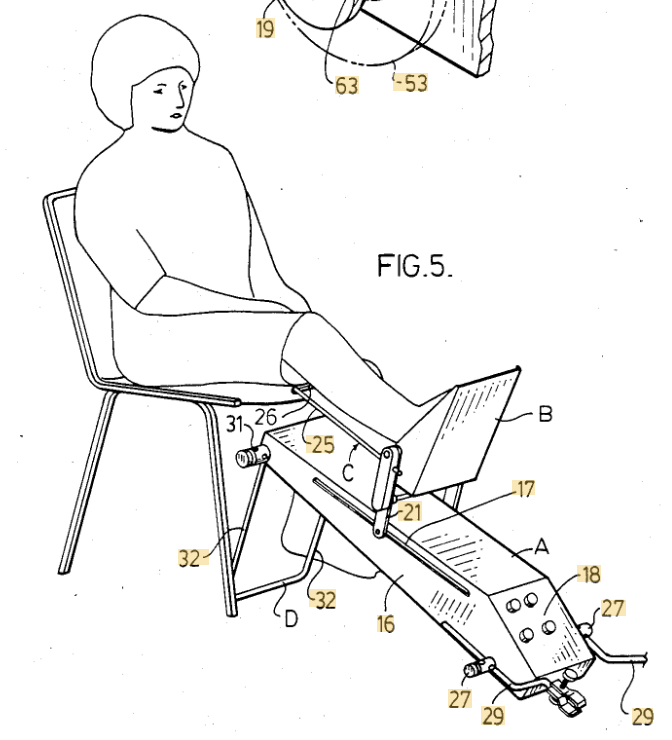
\includegraphics[width=0.54\linewidth]{US4637379A.png}
  \caption{US4637379A device for continuous passive motion of leg joints.}
  \label{fig:US4637379A}
\end{figure}

\subsection{Mechanism kinematics}
\begin{figure}[H]
  \centering
  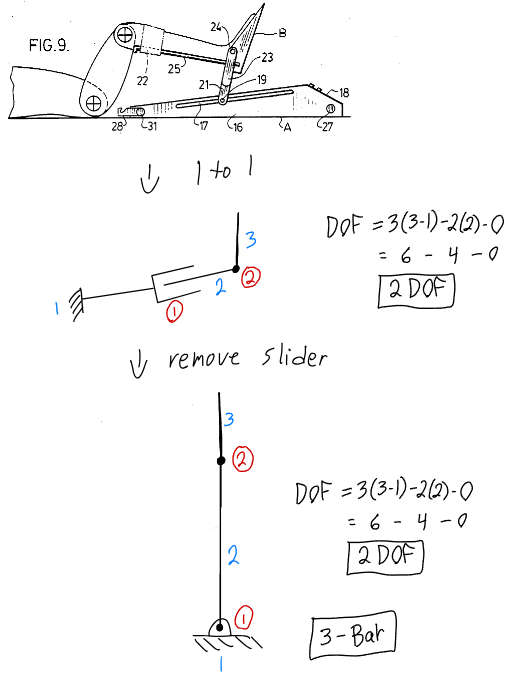
\includegraphics[width=0.54\linewidth]{../Kinematic Mechanism Images/4637379.png}
  \caption{Kinematics diagram for US4637379A device for imparting continuous passive motion to leg joints.}
  \label{fig:US4637379A_kinematics}
\end{figure}

\subsection{Degrees of Freedom}
\[
\begin{aligned}
DOF &= 3(n-1) - 2f_1 - f_2 \\
DOF &= 3(3-1) - 2(2) - 0 \\
DOF &= 2
\end{aligned}
\]

The mechanism is simply a 3 bar linkage with 2 degrees of freedom.

\subsection{Observations}
This patent discloses a hybrid actuation structure in which a motor driven carriage executes linear reciprocation along a base, and that motion is translated into combined longitudinal and arcuate displacement of a foot rest. The design enables selectively mobilizing the hip and knee together (with the ankle held) or mobilizing the ankle alone (with knee/hip fixed) by using a spacing or locking frame to change the pivot constraints. By altering the path constraints, it switches between two modes of articulation. closed-loop control to regulate stroke length independent of carriage position. The device also provides adjustable supports and mounting legs to align the base relative to the patient. Despite this flexibility, its reliance on a rigid frame and discrete mode switching may limit smooth transitions and patient comfort under varying anatomical geometries.

\subsection{Opportunities for Improvement}
One opportunity is to replace the discrete mode-switching between joint combinations with a continuously adaptive kinematic coupling. For example, a mechanism that gradually shifts the pivot locus rather than fully locking or unlocking frames. This would smooth transitions and better accommodate patient specific joint behavior.

\section{US4665899A: Apparatus for Articulating the Knee and Hip Joints}
\subsection{Description}
Apparatus that articulates knee and hip simultaneously using dual-arm linkages spanning a reciprocating carriage and base; adjustable arm lengths accommodate different limb sizes while a foot support pivots on the carriage.
\subsection{Images}
\begin{figure}[H]
  \centering
  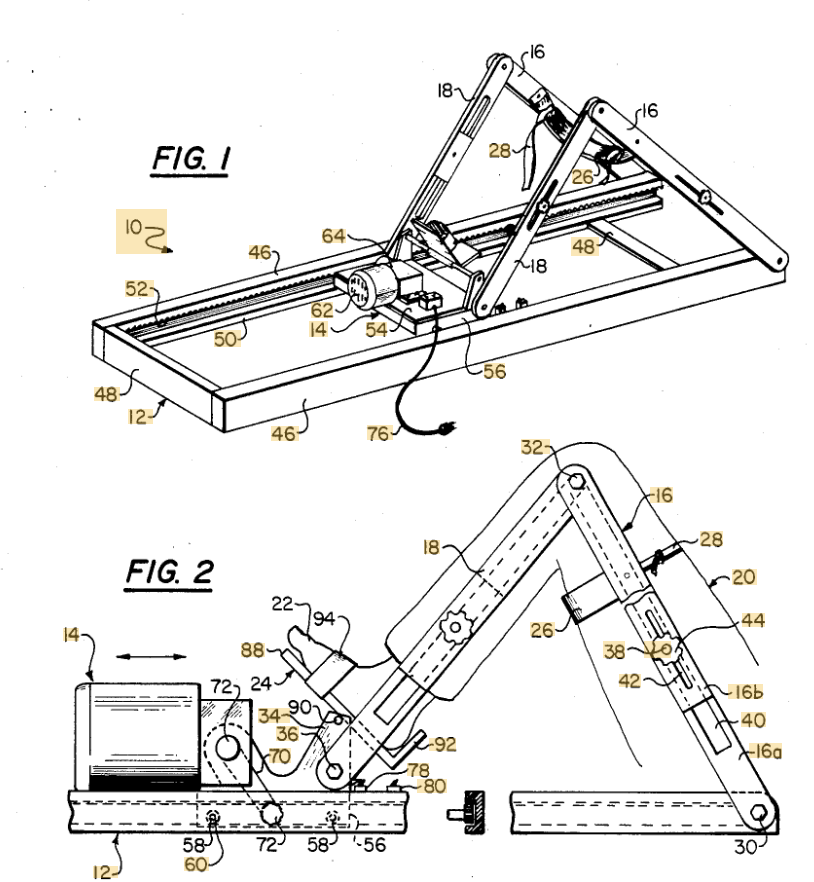
\includegraphics[width=0.54\linewidth]{US4665899A.png}
  \caption{US4665899A apparatus for coordinated knee and hip joint articulation.}
  \label{fig:US4665899A}
\end{figure}

\subsection{Mechanism kinematics}
\begin{figure}[H]
  \centering
  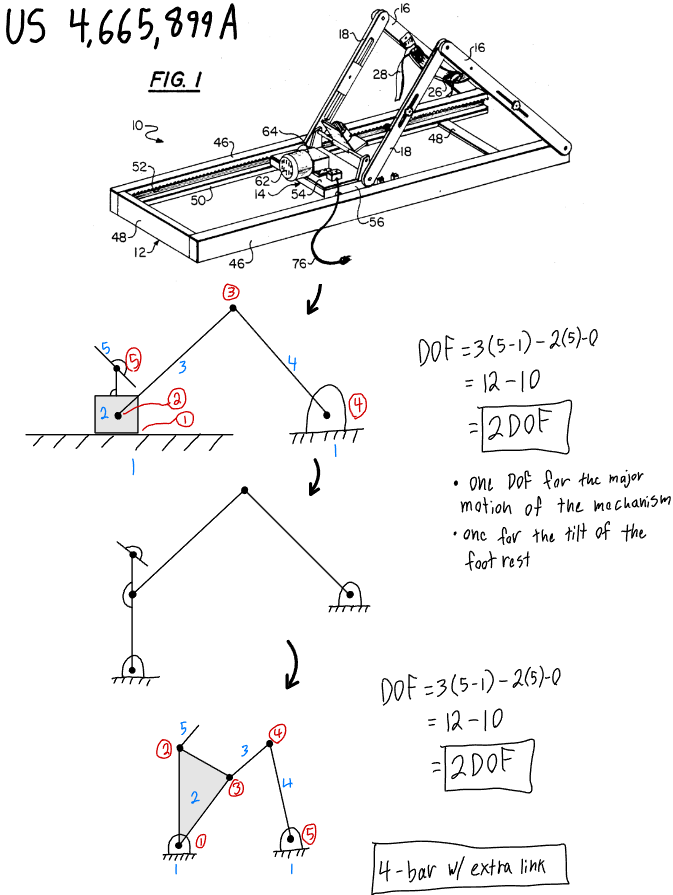
\includegraphics[width=0.54\linewidth]{../Kinematic Mechanism Images/4665899.png}
  \caption{Kinematics diagram for US4665899A apparatus for articulating the knee and hip joints.}
  \label{fig:US4665899A_kinematics}
\end{figure}

\subsection{Degrees of Freedom}
\[
\begin{aligned}
DOF &= 3(n-1) - 2f_1 - f_2 \\
DOF &= 3(5-1) - 2(5) - 0 \\
DOF &= 2
\end{aligned}
\]

The mechanism is a 4 bar linkage with an extra link added.

\subsection{Observations}
This patent describes a dual arm linkage system in which a carriage reciprocates along a fixed base, with a first pair of arms pivoting from the base and a second pair connecting to the carriage, creating a four bar like structure spanning the leg. The foot is mounted on a pivoting support on the carriage, and the thigh is cradled by supports between the first arms. Reciprocal motion of the carriage articulates both the knee and hip simultaneously in a coordinated path. The device also includes adjustable arm lengths (via sliding members) to accommodate different thigh lengths and patient sizes. The floating coupling of the thigh cradle to the arms allows relative rotational movement, which helps reduce misalignment stress. Its structural approach is robust and better suited to capture the coupled kinematics of hip knee motion than purely single pivot designs.

\subsection{Opportunities for Improvement}
The adjustable arm length elements could be enhanced with indexable detents or tool-less locking to speed up clinical configuration. The floating coupling could be further refined with compliant joints or flexure elements to absorb minor misalignment without force spikes. Finally, advancing the actuation system with a smooth motion profile (cam or variable transmission) instead of straight reciprocity could reduce abrupt transitions and better mimic physiological joint movement.

\section{WO2011119902A1: Continuous Passive Motion Device}
\subsection{Description}
Seated-format CPM using a cable-drum drive to reciprocate a sliding member that pivots a foot pedal; heel position is adjustable and a user control switch sets motion direction, enabling compact home/clinic use.
\subsection{Images}
\begin{figure}[H]
  \centering
  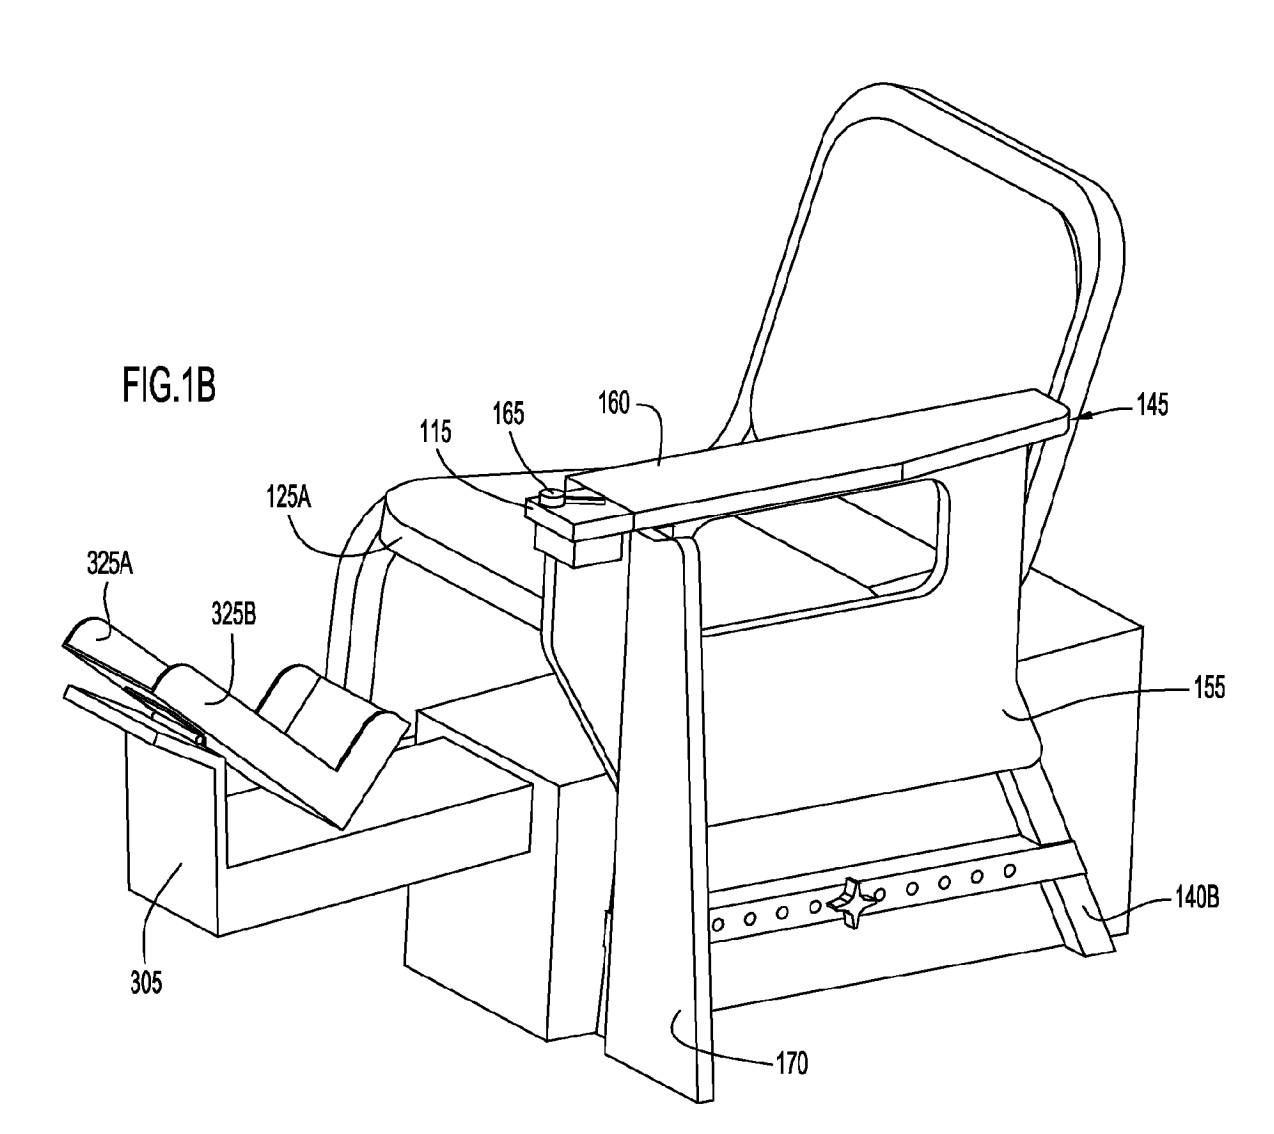
\includegraphics[width=0.54\linewidth]{WO2011119902A1.png}
  \caption{WO2011119902A1 modern continuous passive motion device.}
  \label{fig:WO2011119902A1}
\end{figure}

\subsection{Mechanism kinematics}
\begin{figure}[H]
  \centering
  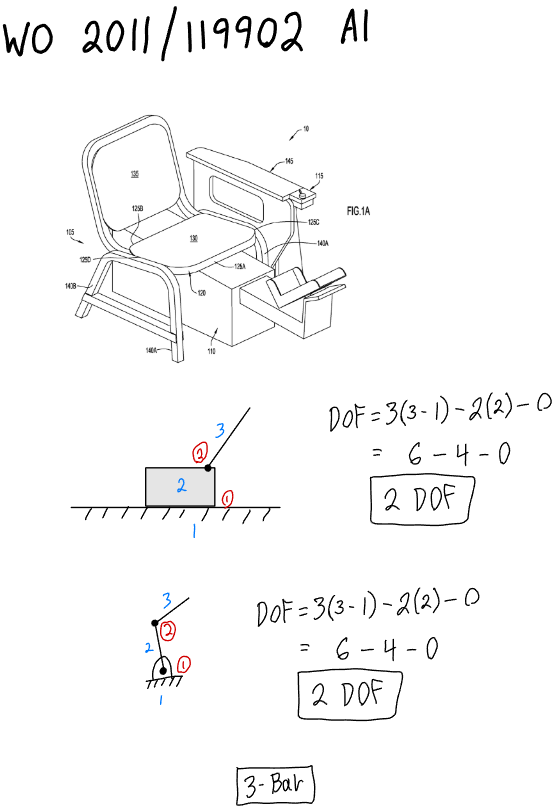
\includegraphics[width=0.54\linewidth]{../Kinematic Mechanism Images/WO 2001_119902.png}
  \caption{Kinematics diagram for WO2011119902A1 continuous passive motion device.}
  \label{fig:WO2011119902A1_kinematics}
\end{figure}

\subsection{Degrees of Freedom}
\[
\begin{aligned}
DOF &= 3(n-1) - 2f_1 - f_2 \\
DOF &= 3(3-1) - 2(2) - 0 \\
DOF &= 2
\end{aligned}
\]

The mechanism is a 3 bar linkage with 2 degrees of freedom.

\subsection{Observations}
This international patent presents a CPM arrangement in which a patient remains seated and a sliding member moves longitudinally to drive a pivoting foot pedal mechanism. The drive is implemented via a cable wrapped around a drum, driven by a reversible motor, with the cable pulling the slide back and forth over pulleys. The foot pedal is pivotally attached to the slide, enabling adjustment for different heel positions. A control switch interface allows the patient to set motion direction. The design shifts away from full-leg support systems to a more compact seated format, potentially increasing usability and convenience for home or clinical settings. However, the use of cable-driven actuation may introduce slack, friction, or backlash in the system, and the kinematics are limited by the fixed cable path and pulley geometry.

\subsection{Opportunities for Improvement}
To enhance this design, replacing or augmenting the cable drum drive with a stiffer actuation system would reduce compliance, backlash, and maintenance. Adjustable or interchangeable cable-guiding pulleys or routing paths could tailor motion profiles to individual patients, improving ergonomics. Lastly, a smoother motion profile (gradual acceleration/deceleration) could be implemented to reduce abrupt transitions and patient discomfort.

\clearpage
\section*{Appendix: Mechanism Summary Table}
\begin{table}[H]
  \centering
  \small
  \caption{Summary of patent mechanisms and kinematic properties}
  \begin{tabular}{|l|l|c|c|c|c|c|l|l|}
    \hline
    Page & Patent No. & Links & $f_2$ & $f_1$ & DOF & BKC Links & Chain/Structure & Task \\
    \hline
    \pageref{fig:US4509509A} & US4509509A & 7 & 0 & 8 & 2 & 7 & Watt II + extra link & Motion \\
    \hline
    \pageref{fig:US4549534A} & US4549534A & 7 & 0 & 10 & 1 & 6 & Watt II & Motion \\
    \hline
    \pageref{fig:US4566440A} & US4566440A & 14 & 0 & 19 & 1 & 12 & Watt I & Motion \\
    \hline
    \pageref{fig:US4974830A} & US4974830A & 4 & 0 & 4 & 1 & 4 & 4-Bar & Motion \\
    \hline
    \pageref{fig:US5333604A} & US5333604A & 9 & 0 & 11 & 2 & 9 & Watt II + 4-Bar & Motion \\
    \hline
    \pageref{fig:US6267735B1} & US6267735B1 & 6 & 0 & 7 & 1 & 6 & Watt I & Motion \\
    \hline
    \pageref{fig:US6325770B1} & US6325770B1 & 5 & 0 & 6 & 0 & 5 & Watt I & Motion \\
    \hline
    \pageref{fig:US5252102A} & US5252102A & 4 & 0 & 4 & 1 & 4 & 4-bar & Function \\
    \hline
    \pageref{fig:US4492222A} & US4492222A & 6 & 0 & 7 & 1 & 6 & Watt I & Motion \\
    \hline
    \pageref{fig:US10272291B2} & US10272291B2 & 2 & 0 & 1 & 1 & 2 & Slider & Path \\
    \hline
    \pageref{fig:US4603687A} & US4603687A & 8 & 0 & 10 & 1 & 8 & Watt I + extra dyad & Motion \\
    \hline
    \pageref{fig:US5239987A} & US5239987A & 4 & 0 & 4 & 1 & 4 & 4-bar & Motion \\
    \hline
    \pageref{fig:US4546763A} & US4546763A & 6 & 1 & 6 & 1 & 6 & Watt I & Motion \\
    \hline
    \pageref{fig:US4637379A} & US4637379A & 3 & 0 & 2 & 2 & 3 & 3-bar & Motion \\
    \hline
    \pageref{fig:US4665899A} & US4665899A & 5 & 0 & 5 & 2 & 5 & 4-bar like & Motion \\
    \hline
    \pageref{fig:WO2011119902A1} & WO2011119902A1 & 3 & 0 & 2 & 2 & 3 & 3-bar & Path \\
    \hline
  \end{tabular}
\end{table}

\end{document}


